\documentclass{article}
\usepackage[utf8]{inputenc}
\usepackage{amsfonts, amsmath, amssymb, graphicx, epstopdf, mathtools, varioref, comment, afterpage, float, url, subfig, algorithmic, algorithm, pgf, soul, booktabs, verbatim, bbm, flafter, color, multirow, units, tabularx,scalerel}
\usepackage[round]{natbib}
\usepackage[left=0.8in,top=0.8in,right=0.8in,bottom=0.8in]{geometry}
\usepackage{mathrsfs}

\urldef\myurl\url{http://data.dft.gov.uk/driving-licence-data/Driving-Licence-Data-User-Guide%20%288%29%20June%202017%20version.docx}

\usepackage{footnote}
\makesavenoteenv{tabular}
\makesavenoteenv{table}

\usepackage{tikz}
\usetikzlibrary{shapes}
\usetikzlibrary{fit}
\usetikzlibrary{chains}
\usetikzlibrary{arrows}

\usepackage{soul}
\usepackage{color}

\newcommand{\hlpink}[1]{{\sethlcolor{pink}\hl{#1}}}

% Latent node
\tikzstyle{latent} = [circle,fill=white,draw=black,inner sep=1pt,
minimum size=20pt, font=\fontsize{10}{10}\selectfont, node distance=1]
% Observed node
\tikzstyle{obs} = [latent,fill=gray!25]
% Marginal node
\tikzstyle{margin} = [latent,dashed,draw=gray!40!black]
% Constant node
\tikzstyle{const} = [rectangle, inner sep=0pt, node distance=1]
% Factor node
\tikzstyle{factor} = [rectangle, fill=black,minimum size=5pt, inner
sep=0pt, node distance=0.4]
% Deterministic node
\tikzstyle{det} = [latent, diamond]

% Plate node
\tikzstyle{plate} = [draw, rectangle, rounded corners, fit=#1]
% Invisible wrapper node
\tikzstyle{wrap} = [inner sep=0pt, fit=#1]
% Gate
\tikzstyle{gate} = [draw, rectangle, dashed, fit=#1]

% Caption node
\tikzstyle{caption} = [font=\footnotesize, node distance=0] %
\tikzstyle{plate caption} = [caption, node distance=0, inner sep=0pt,below left=5pt and 0pt of #1.south east] %
\tikzstyle{factor caption} = [caption] %
\tikzstyle{every label} += [caption] %

\tikzset{>={triangle 45}}

% \edge [options] {inputs} {outputs}
\newcommand{\edge}[3][]{ %
  % Connect all nodes #2 to all nodes #3.
  \foreach \x in {#2} { %
    \foreach \y in {#3} { %
      \path (\x) edge [->,#1] (\y) ;%
      %\draw[->,#1] (\x) -- (\y) ;%
    } ;
  } ;
}

% \factor [options] {name} {caption} {inputs} {outputs}
\newcommand{\factor}[5][]{ %
  % Draw the factor node. Use alias to allow empty names.
  \node[factor, label={[name=#2-caption]#3}, name=#2, #1,
  alias=#2-alias] {} ; %
  % Connect all inputs to outputs via this factor
  \factoredge {#4} {#2-alias} {#5} ; %
}

% \plate [options] {name} {fitlist} {caption} {location}
\newcommand{\plate}[4][]{ %
  \node[wrap=#3] (#2-wrap) {}; %
  \node[plate caption=#2-wrap] (#2-caption) {#4}; %
  \node[plate=(#2-wrap)(#2-caption), #1] (#2) {}; %
}



\title{Modelling casualties}
\begin{document}
\maketitle

\abstract{We present a predictive model for the numbers of fatalities and injuries resulting from road-traffic collisions in England, itemised by the specifics of the collision. We estimate numbers by calculating risks: the number of casualties (injuries or fatalities), per km travelled by the casualty, per km travelled by the striker, per year. To estimate the exposure (the distance travelled), we use numerous sources of administrative data. We estimate one rate per road type, per casualty severity, per casualty demographic group, per striker demographic group, per casualty travel mode, per striker travel mode, per year.}

\section{Introduction}

Death and disability due to road-traffic crashes ... . We predict injury and fatality rates (the number per distance travelled) as functions of the specifics of the crash. We are interested in the role of the striking-vehicle covariates as well as the pattern of injury rates as they pertain to the casualties of crashes \citep{Feleke2017,Scholes2017a}.

The primary data source for our model of road-traffic injuries and fatalities is the Stats19 database. These are records of all road-traffic injuries reported to the police, where each entry (row) corresponds to one injury or fatality, which we refer to in general as ``casualties''. We use this source to count the total number of events of each type.

We group the records into ``types'' according to the specifications of the crash and resulting casualties. We refer to these specifics as predictors or covariates. The predictors we use are: casualty mode, casualty demographic group (casualty age and casualty gender), casualty severity, strike mode, striker demographic group (striker age and striker gender), road type, and year. %The ``striker'' is defined as the driver of the largest other vehicle in the collision. 
They are listed in Table \ref{indices}, along with the possible values they take in the dataset. Then we define the multidimensional array of casualty counts as $I_{a_{\text{cas}},g_{\text{cas}},m_{\text{cas}},a_{\text{str}},g_{\text{str}},m_{\text{str}},c,t,y}$.

The casualty counts are to be understood in terms of exposure: what amount of exposure to risk led to how many casualties. We measure exposure in terms of distance travelled. We must therefore estimate the distance travelled by each demographic subgroup by each mode on each road type in each year. %These data are not readily available, and must be constructed from numerous different sources.

Then we describe the casualty counts as a smooth function of the predictors, offset by the distance travelled per casualty and per striker. We use a regression model to relate the covariates to the casualty counts in a smooth manner that allows the sharing of support across the (sometimes sparse) counts of casualties. 

\hl{Do we, in parallel, present a model for no-other-vehicle crashes, which would include pedestrian falls from a different source, and has as predictors only casualty mode, casualty demographic group (casualty age and casualty gender), casualty severity, road type, and year?} \citep{Methorst2017,Ward2005}

A future development to our methodology would be to include a spatial component, as in \citet{Boulieri2016}. 

The rest of the paper is structured as follows. In Section \ref{exp} we describe how we construct the distances travelled for the population in such a way that it provides a plausible offset for the casualty counts. In Section \ref{injuries} we describe the processing of the casualty data. In Section \ref{regression} we describe the regression modelling. In Section \ref{results} we present some results: the estimated rates of injury and fatality.

\begin{table}[ht]
\begin{center}
\caption{Indices used to denote model variables.}
\begin{tabular}{lll}
\label{indices}
Index & Name & Values \\
\hline
\multicolumn{3}{c}{\textit{Predictors}}\\
\hline
$a$ & Age groups & 0--105\\
$c$ & Casualty severity & Fatal \\
& & Serious \\
& & Slight \\
$g$ & Gender & Female, male \\
$m$ & Transport modes& Pedestrian, cyclist,\\
& & car/taxi, motorbike, \\
& & bus, HGV, LGV \\
$t$ & Road type & Motorway \\
& & A \\
& & B, C, unclassified \\
$y$ & Year & 2005--2015\\
\hline
\multicolumn{3}{c}{\textit{Other indices}}\\
\hline
$r$& Role & Casualty (cas) \\
& & Striker (str) \\
$s$ & Scenarios & (User specified)\\
$z$ & Passenger& No (0) \\
& & Yes (1) \\
\hline
\end{tabular}
\end{center}
\end{table}


\section{Exposure: distance travelled}\label{exp}

Our exposure to risk is defined as the distance travelled by the casualty group and the distance travelled by the striker group, stratified by the relevant covariates. We define these as $A_{a,g,m,t,y}^{\text{(cas)}}$ and $A_{a,g,m,t,y}^{\text{(str)}}$. $A_{a,g,m,t,y}$ denotes the total distance travelled by people in demographic group $\{a,g\}$, by mode $m$, on road type $t$, in year $y$. $A_{a,g,m,t,y}^{\text{(cas)}}$ and $A_{a,g,m,t,y}^{\text{(str)}}$ might differ (a) in terms of having different age-group categories $a$, and (b) due to the inclusion of passengers in the former but not the latter. 

As these are not known values, we use a number of data sources to estimate them.  We construct them via a complete array, $B$, that includes all covariates: $B=B_{a,g,m,t,y,z}$. This includes an additional index, $z$, that denotes whether travel is taken as a passenger or not. This allows us to estimate both  the number of people and the number of vehicles on the roads. Then we define the casualty exposure as $$A_{a,g,m,t,y}^{\text{(cas)}}=\sum_{z=0,1}B_{a,g,m,t,y,z}$$ and the striker exposure as $$A_{a,g,m,t,y}^{\text{(str)}}=B_{a,g,m,t,y,z=0}.$$

We use the datasets listed in Table \ref{timetraveldata} to construct $B$. First, we use vehicle road--distance data, which estimates the total distance travelled per year per road type by each mode Section \ref{rts}). We take these to be the true totals to which the distances should sum, as they are more objective than survey data with which we combine them. 

The survey data with which we combine them are from the National Travel Survey (Section \ref{nts}). These data provide demographic travel information. By combining these two data sources, we can allocate distances to three road types using a heuristic method so that in total the distance travelled on a road is a fair approximation to the ``true'' total (Section \ref{distribute}). For the subset of groups for which there are no relevant data from the survey we use license data (Section \ref{dvla}). Finally, we smooth the resulting estimates (Section \ref{smooth}).

\begin{table}[h]
\centering
\caption{\small Datasets used to calculate $B_{a,g,m,t,y,z}$}
\begin{tabular}{lp{5cm}lll}
%\begin{tabular}{cll}
Label & Description & Source & Years & Geographical region \\
\hline
$R_{m,t,y}$ & Total miles driven on different road types by vehicle type\footnote{\url{https://www.gov.uk/government/uploads/system/uploads/attachment_data/file/610721/tra4215.ods}} & RTS & 2005--2015 & England \\
$D_{j}$ & Distance travelled on trip $j$ in NTS database & NTS & 2005--2015 & England \\
$L_{a,g,m}$ & License-holder data from the DVLA\footnote{Data for other years are missing and/or improbable. We use license type D (full) and D (auto) for bus drivers and C1E and C1 full and auto for HGV: \myurl} & DVLA & 2015 & GB \\
$N_{a,g,y}$ & License-holder data from the DVLA\footnote{\url{https://www.ons.gov.uk/file?uri=/peoplepopulationandcommunity/populationandmigration/populationestimates/datasets/populationestimatesforukenglandandwalesscotlandandnorthernireland/mid2015/ukandregionalpopulationestimates18382015.zip}} & ONS & 2005--2015 & England \\
\hline
\end{tabular}
\label{timetraveldata}
\end{table}

\subsection{Vehicle road--distance data}\label{rts}

The backbone of our distance data is data from road traffic statistics (RTS) pertaining to road usage. RTS estimates the total distance travelled by each mode on each road type in each year using automatic traffic counters and manual counts. We denote this dataset $R_{m,t,y}$. 

The $R_{m,t,y}$ dataset provides our first constraint: that the ``driver'' component of $B$ is constrained to equal the sum of all distance travelled, i.e. \begin{equation}\label{B}\sum_{a,g,t}B_{a,g,m,t,y,z=0} = \sum_{t}R_{m,t,y}.\end{equation}
 
In what follows, when using datasets to populate $B$, we are subject to the constraint of Equation \ref{B}. 

\subsection{NTS data}\label{nts}

Our primary source for estimated distances travelled is the National Travel Survey (NTS). This is an annual survey that includes a week-long travel diary, completed by \textasciitilde 15,000 participants. It results in a trip-level dataset that forms the basis of our estimate of distance travelled in England.

Each trip in the dataset is taken by a specific individual and by a specified mode, so that the dataset tells us distances travelled categorised by five of the six covariates we require: age, gender, mode, year, and passenger status; i.e., each trip $j$ in the dataset has by definition one of each $a(j)$, $g(j)$, $m(j)$, $y(j)$ and $z(j)$. 

Each trip in the dataset might consist of more than one stage, and therefore more than one mode. The dataset lists the main mode alongside any additional distance travelled by bike or on foot. We add these additional distances as journeys in their own right, and subtract the distance from that travelled by the main mode. The total dataset increases from 3,114,437 entries to 3,161,698 entries.

Each person in the dataset has an assigned weight, according to the perceived representativeness of the person based on their demographic description. Each trip also has a weight, that accounts both for the person taking the trip, and the day on which the trip was made.\footnote{See \url{https://www.gov.uk/government/uploads/system/uploads/attachment_data/file/550854/nts-technical-report-2015.pdf} for details of NTS methodology}

In order to use these data alongside the Stats19 data, we must (a) distribute each trip made by each individual in the population to the three road types, and (b) fill in the gaps: The NTS data lack information on bus drivers and lorry drivers.\footnote{We assume that there are no lorry passengers} ``Bus driver'' is not a mode available to persons filling in the survey, and we find that lorry driving is under-reported, so we instead populate these data using information from the Driver and Vehicle Licensing Agency (Section \ref{dvla}).

\subsubsection{Matching NTS data to RTS data}\label{match}

We find that the NTS data estimate total travel in England to be less than that predicted by RTS (Figure \ref{total}). It is unclear why this should be the case. Assuming RTS data to be more reliable estimates of total distance travelled, and therefore a better indicator of exposure to events that might result in a record in the Stats19 database, we scale NTS trip weights by the following factor:
 $$\rho_{m,y}=\frac{\sum_{t}R_{m,t,y}}{\sum_{\substack{j:m(j)=m,\\
                  y(j)=y,z(j)=0}}\left(D_{j}\cdot W_{j}\right)}\cdot \frac{\sum_{i:y(i)=y}V_{i}}{\sum_{a,g}N_{a,g,y}}$$ 
where $m(j)=m$ and $y(j)=y$ give the mode and year of trip $j$, and $z(j)=0$ restricts us to counting only drivers. $W_j$ are the trip weights from the NTS, $V_i$ the person weights, and $N_{a,g,y}$ are population counts. I.e., for each mode and for each year, we sum the total distance travelled on all road types in the RTS dataset, and sum the distance travelled by all people on all trips from the NTS dataset, divide each by the contributing population to yield an average, and take their ratio as the scaling factor.

\begin{figure}[!b]
\centering
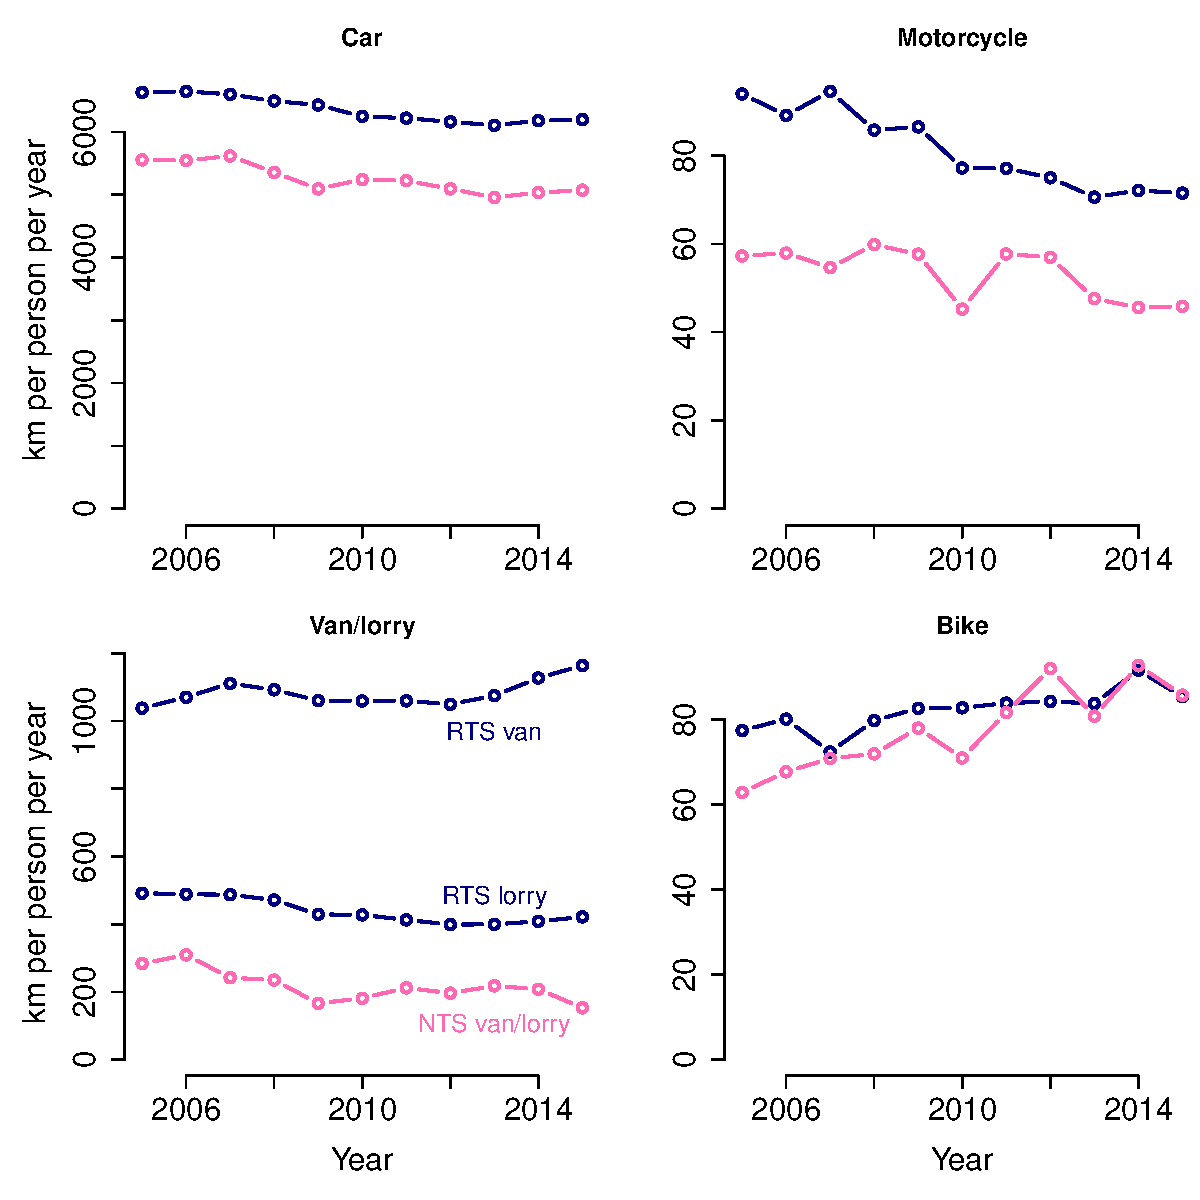
\includegraphics[width=0.6\textwidth]{NTSvsTRA.pdf}
\caption[Estimated average distance travelled per person per year over time.]{\small Estimated average distance travelled per person per year over time. For the RTS estimates, in navy, we use the total distance covered in England divided by the total population in England. For the NTS estimates, in pink, we sum the total distance travelled by mode, weighted according to the NTS-provided trip weights, and divide by the total weight of the participants of the survey.}
\label{total}
\end{figure}


Hence, we are assuming that the RTS data are accurate\footnote{\url{https://www.gov.uk/government/uploads/system/uploads/attachment_data/file/524848/annual-methodology-note.pdf}. Reasons that RTS might overestimate: a) the growth assumption for minor roads; b) if lots of lorry and van drivers reside in Wales and Scotland but cover a lot of ground in England, without a reciprocal effect.} and the NTS data an underestimate; further, we assume that the distances recorded are representative of true distances, and that the person weighting is representative, but the number of trips is not. I.e., we assume that there were more of the same trips, by the same people, that were not reported in the NTS travel diary. Thus we are effectively increasing the trip weight. %\footnote{The NTS methodology (\url{http://doc.ukdataservice.ac.uk/doc/7559/mrdoc/pdf/7559_nts_technical_report_2016.pdf}) includes a procedure for weighting individuals and, subsequently, for weighting trips, in which the individual's weight is included. Then to increase the number of trips per user we increase the trip weight.}  

With this factor, we have an equivalent constraint to Equation \ref{B}, that all the listed journeys should add up to the total distance travelled per mode, per year:
\begin{equation}\sum_{t}R_{m,t,y} = \rho_{m,y} \smashoperator{\sum_{\substack{j:m(j)=m,\\y(j)=y,\\z(j)=0}}}\left(D_{j}\cdot W_{j}\right)\cdot\frac{\sum_{a,g}N_{a,g,y}}{\sum_{i:y(i)=y}V_{i}},\end{equation}
which relates to our target array, $B$, disaggregated also by age and gender, as follows:
\begin{equation}\sum_{t}B_{a,g,m,t,y,z=0} = \rho_{m,y} \smashoperator{\sum_{\substack{j:a(j)=a,\\g(j)=g,m(j)=m,\\y(j)=y,z(j)=0}}}\left(D_{j}\cdot W_{j}\right)\cdot\frac{\sum_{a,g}N_{a,g,y}}{\sum_{i:y(i)=y}V_{i}}.\end{equation}
We assume this to be the true total distance travelled (as a non-passenger) by persons in demographic group $\{a,g\}$ by mode $m$ (excluding bus and lorry) in year $y$.

%Note that $m(j)$ is the main mode of trip $j$. Some trips report also a cycle or walking time, e.g. duration of the journey to the bus stop. These are converted to distances by regressing walking/cycling distances against duration, age and gender for walking/cycling trips and making predictions for the minor-mode trips. These distances are subtracted from the distances of the main-mode trip, and new trips are added with mode labels ``extra walking'' and ``extra cycling''. Both parts for a trip with a resulting major distance less than zero are removed. The net gain in trip number is 46,655.

\subsubsection{Distributing NTS data to road types}\label{distribute}

We now seek some functions $f_{m,t}(D_j)$ that will divide each trip distance $D_j$, taken by mode $m(j)$, into three distances on the three road types, so that the distances add up to $D_j$. Then we can estimate the total distance travelled by a demographic group by a mode on a road type by summing all relevant distances as $$B_{a,g,m,t,y,z=0}= \rho_{m,y}
\smashoperator{\sum_{\substack{j:a(j)=a,\\g(j)=g,m(j)=m,\\y(j)=y,z(j)=0}}}\left(W_j\cdot f_{m(j),t}\left(D_{j}\right)\right)\cdot
\frac{N_{a,g,y}}
{\smashoperator{\sum_{\substack{i:a(i)=a,\\g(i)=g,y(i)=y}}}V_{i}},
\quad  \text{ subject to } \quad\sum_t f_{m(j),t}(D_j)=D_j.$$

We employ a crude division scheme for $f_{m,t}$. We define thresholds $U_{m,t}$ such that the first $U_{m,t=\text{B}}$ km travelled on a journey by mode $m$ are attributed to road type ``B, C, or unclassified'', and the next $U_{m,t=\text{A}}$ are attributed to road type ``A''. Any remaining distance is spent on road type ``motorway'', with the proviso that the remaining distance exceeds $U_{m,t=\text{M}}$ km. It is otherwise added to the total for ``A''. 

More formally, $D_j$ is decomposed to $D_{j,t}$ as follows:
\begin{align}
f_{m(j),t=\text{B}}(D_{j}) &= \min\left(D_j,U_{m(j),t=\text{B}}\right); \\
f_{m(j),t=\text{A}}(D_{j}) &=\left\{\begin{array}{lr} 
0 & \text{if } D_j\leq U_{m(j),t=\text{B}} \\
D_j-U_{m(j),t=\text{B}} & \text{if } U_{m(j),t=\text{B}}< D_{j}\leq\sum_tU_{m(j),t}\\
U_{m(j),t=\text{A}} & \text{if } D_{j}>\sum_tU_{m(j),t} \\
\end{array}\right.\\
f_{m(j),t=\text{M}}(D_{j}) &=\left\{\begin{array}{lr} 
0 & \text{if } D_j\leq \sum_tU_{m(j),t} \\
D_j-\sum_{t\in\{B,A\}}U_{m(j),t} & \text{if } D_{j}>\sum_tU_{m(j),t} \\
\end{array}\right.
\end{align}

We propose the following heuristic values for $U_{m,t}$ (note that we preclude any cyclist travel on motorways):
\begin{equation}\begin{array}{r|ccc}
U_{m,t} & t=\text{B}&t=\text{A} &t=\text{M} \\
\hline
m=\text{bike} & 9 & 80 & \max_j(D_j) \\
m=\text{car} & 6.5 & 40 & 5 \\
m=\text{motorcycle} & 12 & 60 & 5 \\
m=\text{van} & 10 & 50 & 5 \\
\end{array}\end{equation}

We use these functions to distribute all trips in the NTS dataset, regardless of passenger status. As we have no data for pedestrian trips, we distribute them as $U_{m,t=B}=3$ with the remaining distance attributed to A roads, and taxi, minicab and bus trips are distributed as car trips.

Figure \ref{carMF30} shows how $f_{m,t}$ distributes car journeys differently from how they would be distributed were we to apportion each journey according to the same (mode-specific) proportions. We see that, as car journeys taken by males tend to be longer, more of the distance is attributed to motorways, whereas for females, where there are more short journeys, more of the distance travelled is attributed to B, C and unclassified roads.

\begin{figure}[H]
\centering
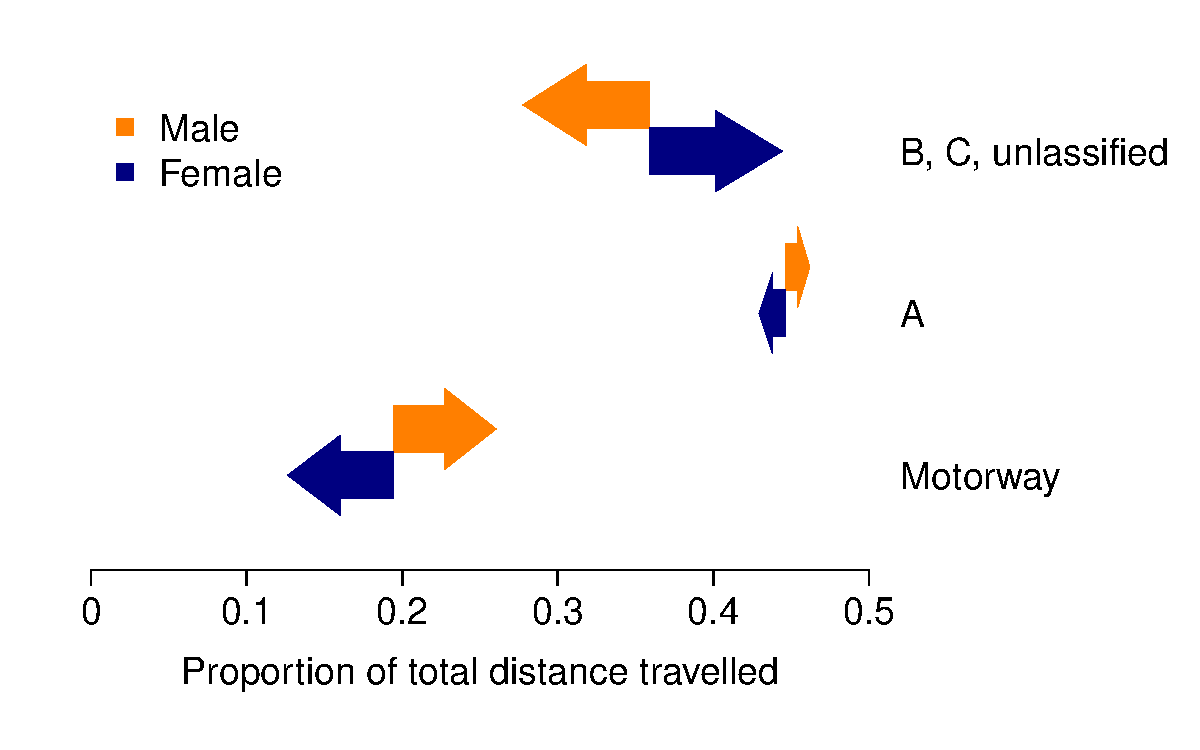
\includegraphics[width=0.5\textwidth]{carMF30.pdf}
\caption[Proportion of total distance travelled by car by male and female 30--39 year olds on each road type.]{\small Proportion of total distance travelled by car by male and female 30--39 year olds on each road type: the ratio of car distance on road type $m$ to car distance on all road types. At arrow origins, the proportion is the same as the total car--road proportions according to the RTS. At arrows points are the proportions when road distances are distributed according to the function $f_{m,t}$. Note that the distributions at the origins are the same for male and female, but differ at the points.}
\label{carMF30}
\end{figure}


\subsection{DVLA data}\label{dvla}

NTS data do not provide useful information on lorry travel (Figure \ref{total}). We therefore assume all NTS ``van/lorry'' trips to be van trips, and we use a separate data source for lorry travel. We use the same method to estimate bus driver travel, i.e. the total distance travelled by buses (whereas the NTS data provide information on bus \text{passengers}).

The RTS-provided estimates for total bus and HGV travel are used directly to understand the total distances travelled by the vehicles. These distances are distributed among the population according to use license-holder data from the DVLA as follows:
\begin{equation}
B_{a,g,m\in\{\text{bus,HGV}\},t,y,z=0}  = \frac{L_{a,g,m\in\{\text{bus,HGV}\}}}{\sum_{a,g}L_{a,g,m\in\{\text{bus,HGV}\}}}\cdot R_{m\in\{\text{bus,HGV}\},t,y}.
\end{equation}

\subsection{Resulting annual travel distances \& smoothing}

Summaries of the resulting annual travel distances are shown in Figures \ref{NTStrajectories} and \ref{NTStrajectoriesperson}. Note the unstable behaviour of light goods distances in Figure \ref{NTStrajectories} towards 2015; this pattern is not reflected in RTS data. It suggests that a better road-partitioning method is required for light goods vehicles. 

Note also the noisiness in motorcycle data in Figure \ref{NTStrajectoriesperson}. There are numerous entries with a total distance of 0 in this set which we believe to be inaccurate representation of the true amount of travel. For example, if we have $B_{a,g,m,t,y,z}=0$ for $a=30$, $g=\text{female}$, $m=\text{motorcycle}$, $t=\text{A road}$, $y=2010$ and $z=\text{driver}$, but we have $B_{a,g,m,t,y,z}>0$ for the same $\{a,g,m,t,z\}$ and $y\in\{2008,2009,2011,2012\}$, then we might assume that, in reality, $B_{a,g,m,t,y=2010,z}>0$.

\begin{figure}[H]
\centering
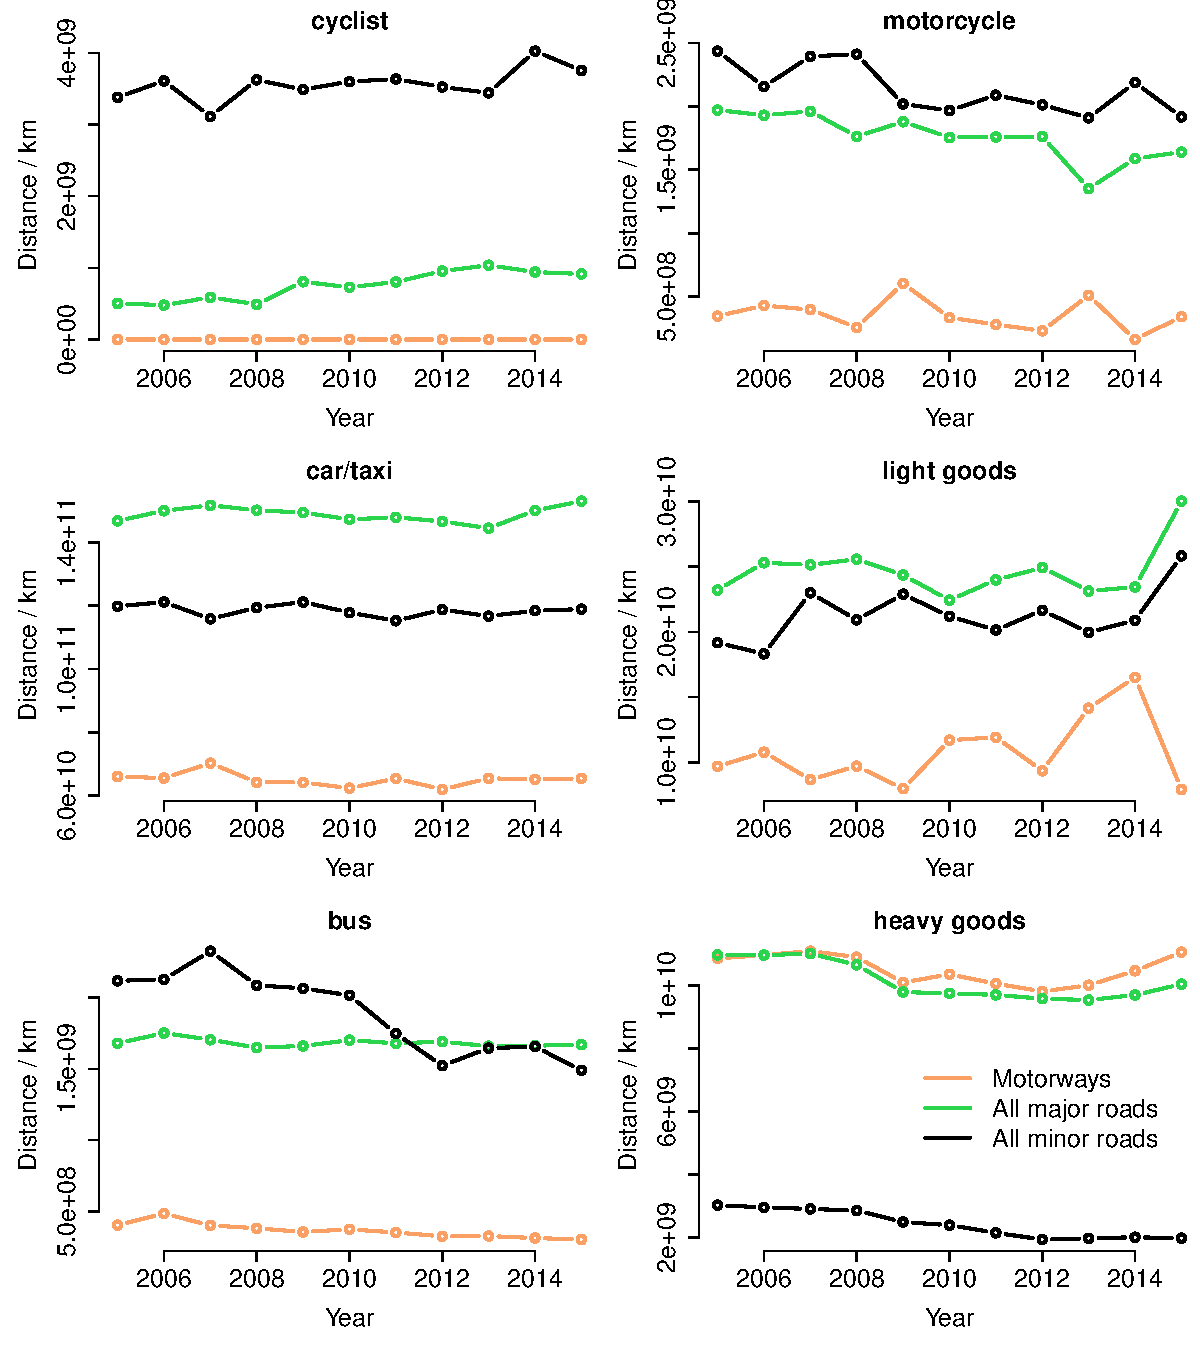
\includegraphics[width=0.6\textwidth]{NTStrajectories.pdf}
\caption{\small Estimated total distance travelled by mode and road type over time.}
\label{NTStrajectories}
\end{figure}

\begin{figure}[H]
\centering
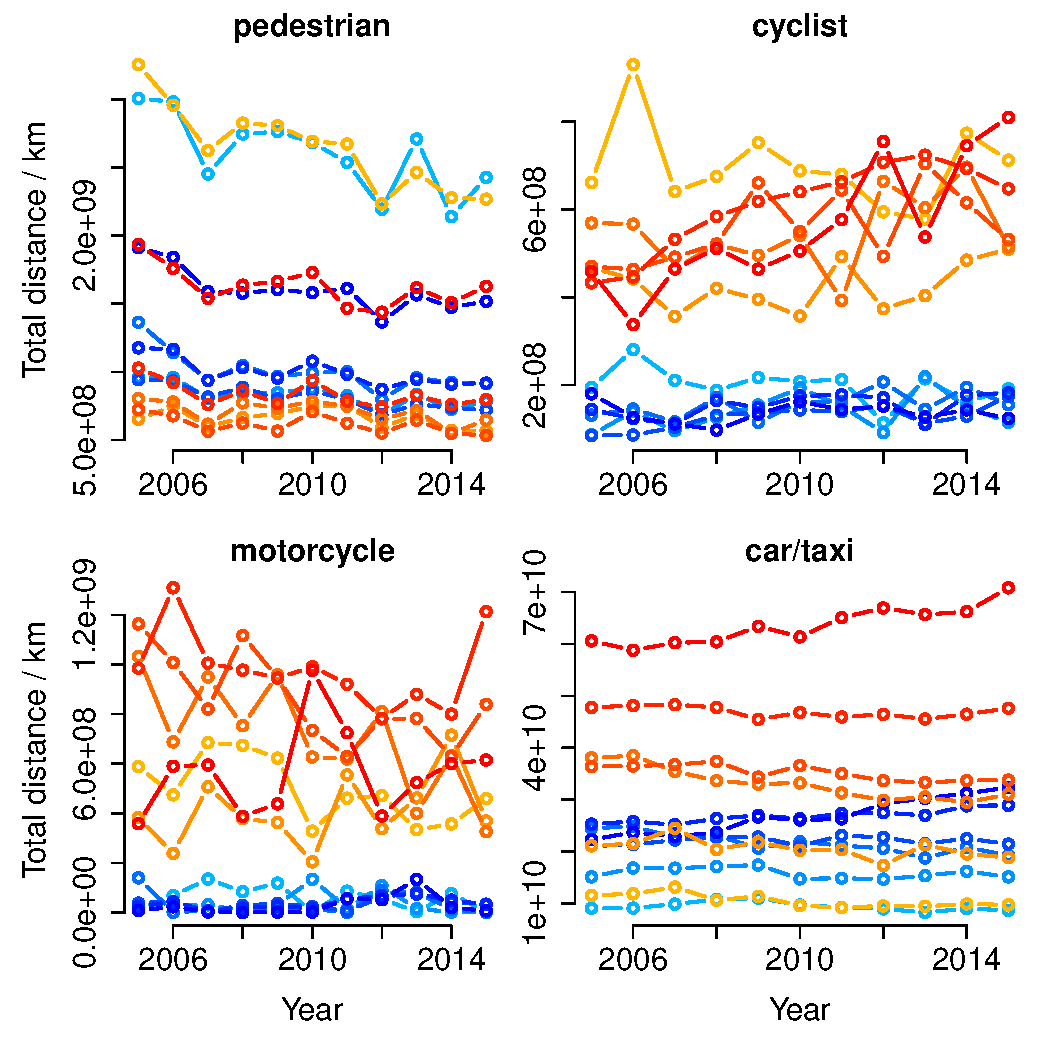
\includegraphics[width=0.5\textwidth]{NTStrajectoriesperson.pdf}
\caption{\small Estimated total distance driven by mode and demographic over time. Colours blue and red indicate female and male groups, respectively. Lighter shades indicate younger age groups. The median ages of the age groups are: 20, 27, 35, 42, 50, and 64.}
\label{NTStrajectoriesperson}
\end{figure}

\subsubsection{Smoothing}\label{smooth}

To correct for errant zero entries, we smooth these data, shown for drivers and passengers in Figures \ref{smoothdrive} and \ref{smoothpass}. At the same time we also smooth out noisiness of similar provenance. In doing so we are estimating what we believe to be the true exposure of the population to casualty risk.

We use a logistic model to decide if a distance should be zero or non-zero, expecting, for example, that the distance driven by children is zero. We then apply a log-normal regression to all non-zero values. We then predict distances for all rows for which the probability of being non-zero is greater than 0.1.

The model for the distances, $B_{a,g,m,t,y,z}$, is
\begin{align}
\log({B}_{a,g,m,t,y,z}) \sim & \mathcal{N}(\log(\mu_{a,g,m,t,y,z}),\sigma^2)\label{smoothEq}\\
\log(\mu_{a,g,m,t,y,z}) =& f(m:(\mathcal{S}_1(y)+g\times z+\mathcal{S}_1(y):\mathcal{S}_8(a)+g:(\mathcal{S}_6(a)+t:z+t:\mathcal{S}_3(a):z)))
\end{align}
where $\mathcal{S}_d$ is a smooth spline with $d$ degrees of freedom.

Defining $\pi_{a,g,m,t,y,z}$ as the probability that the true distance is greater than zero, we estimate the smooth distance-travelled array, $\tilde{B}$, as:
$$\tilde{B}_{a,g,m,t,y,z}=\left\{\begin{array}{ll}\pi_{a,g,m,t,y,z}\mu_{a,g,m,t,y,z} & \pi_{a,g,m,t,y,z}>0.1\\ 0 & \pi_{a,g,m,t,y,z} \leq 0.1 \end{array}\right.$$  

Finally, we calculate the exposures as $$A_{a,g,m,t,y}^{\text{(cas)}}=\sum_{z=0,1}\tilde{B}_{a,g,m,t,y,z}\quad\text{and}\quad A_{a,g,m,t,y}^{\text{(str)}}=\tilde{B}_{a,g,m,t,y,z=0}.$$

%The fit is not brilliant, e.g. the blue motorcyclists in Figure \ref{smoothdrive} who aren't in Figure \ref{NTStrajectoriesperson}. Further, I wonder if it would be sensible to smooth at an earlier stage, e.g. Section \ref{match}, as we now have numbers that do not necessarily add up to the RTS totals.

\begin{figure}[H]
\centering
\begin{tabular}{cc}
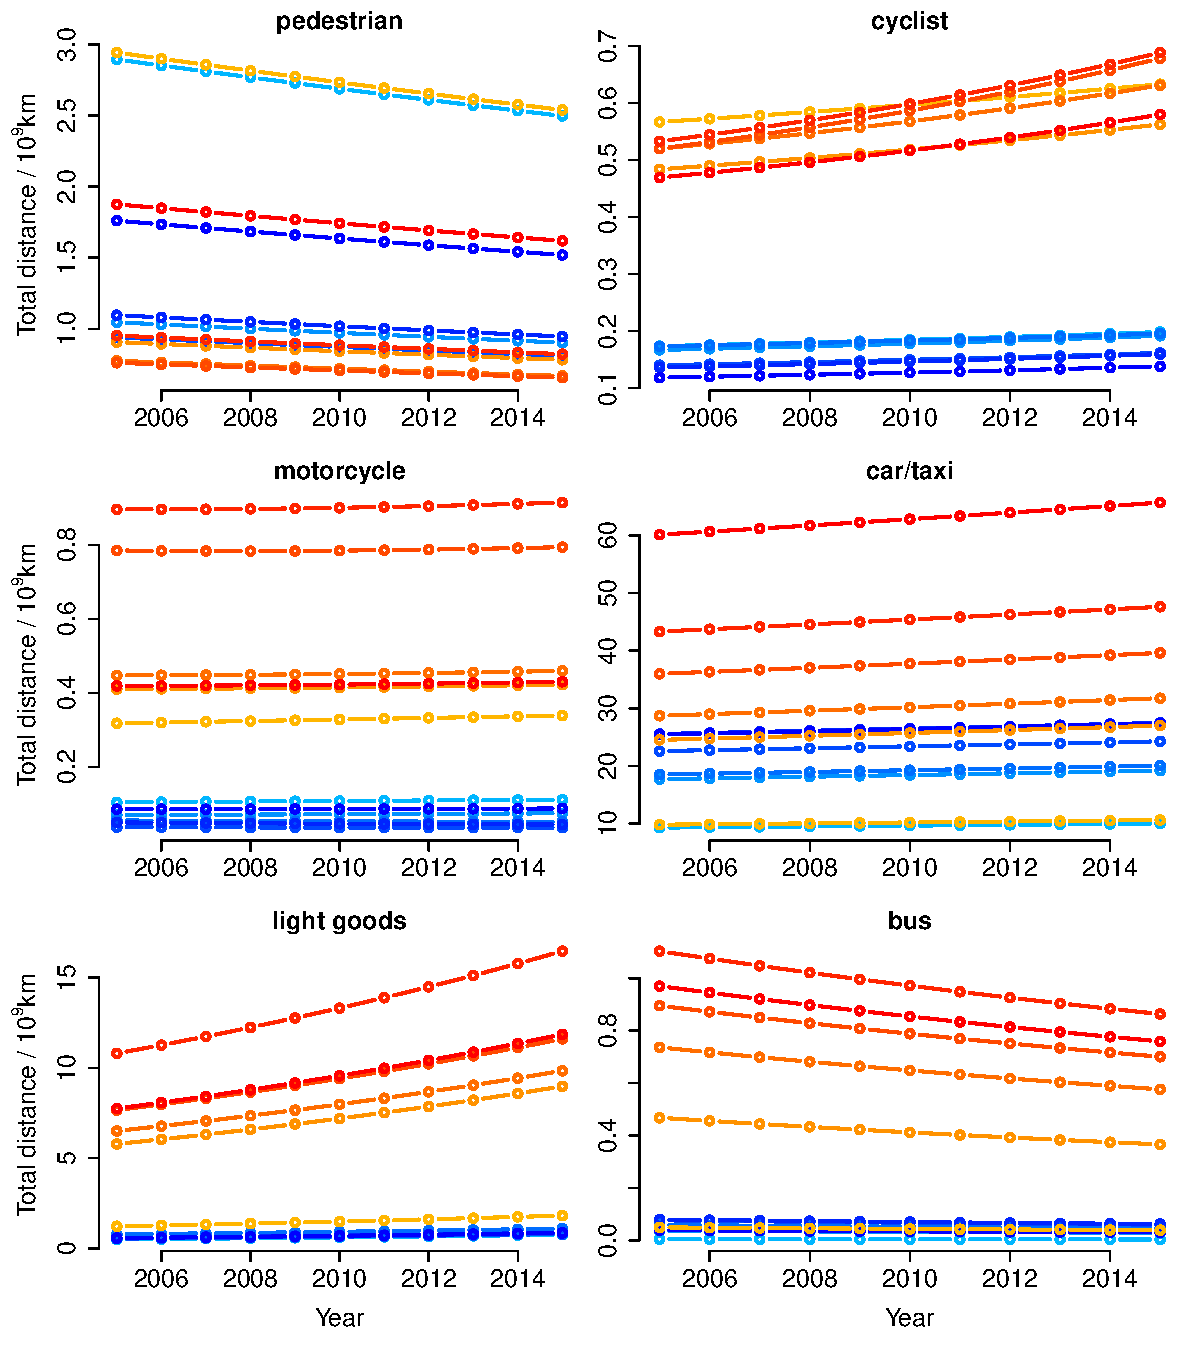
\includegraphics[width=0.45\textwidth]{driverSmooth.pdf}&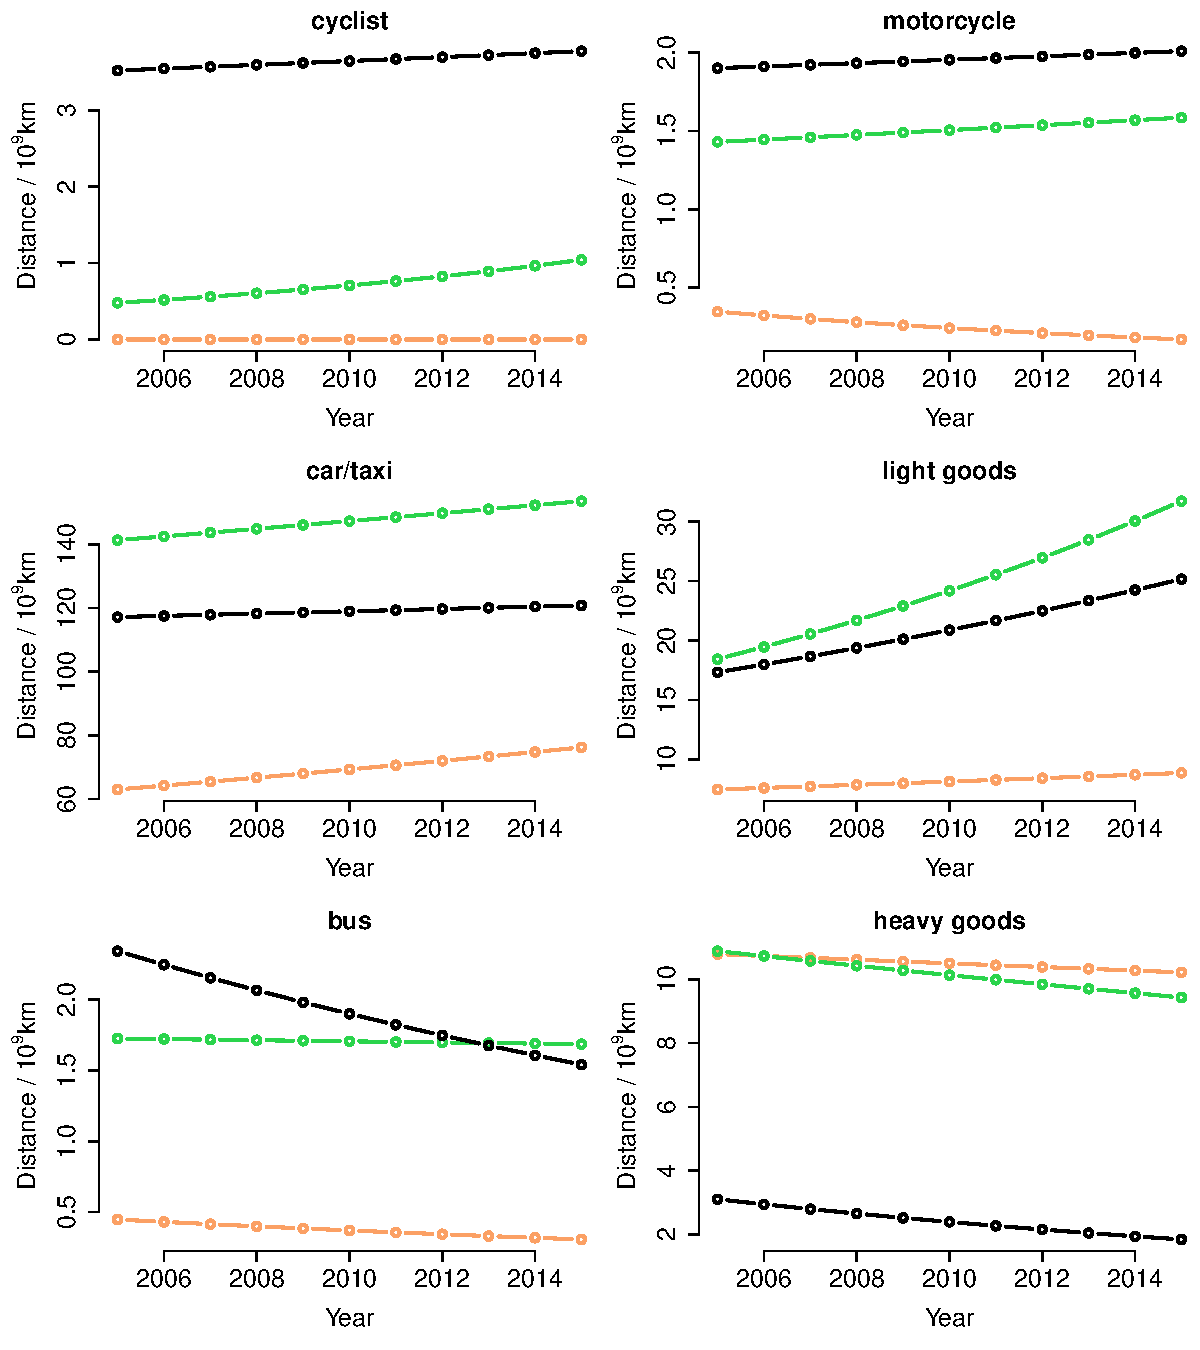
\includegraphics[width=0.45\textwidth]{roadsSmooth.pdf}
\end{tabular}
\caption{\small Smoothed data: drivers.}
\label{smoothdrive}
\end{figure}

\begin{figure}[H]
\centering
\begin{tabular}{cc}
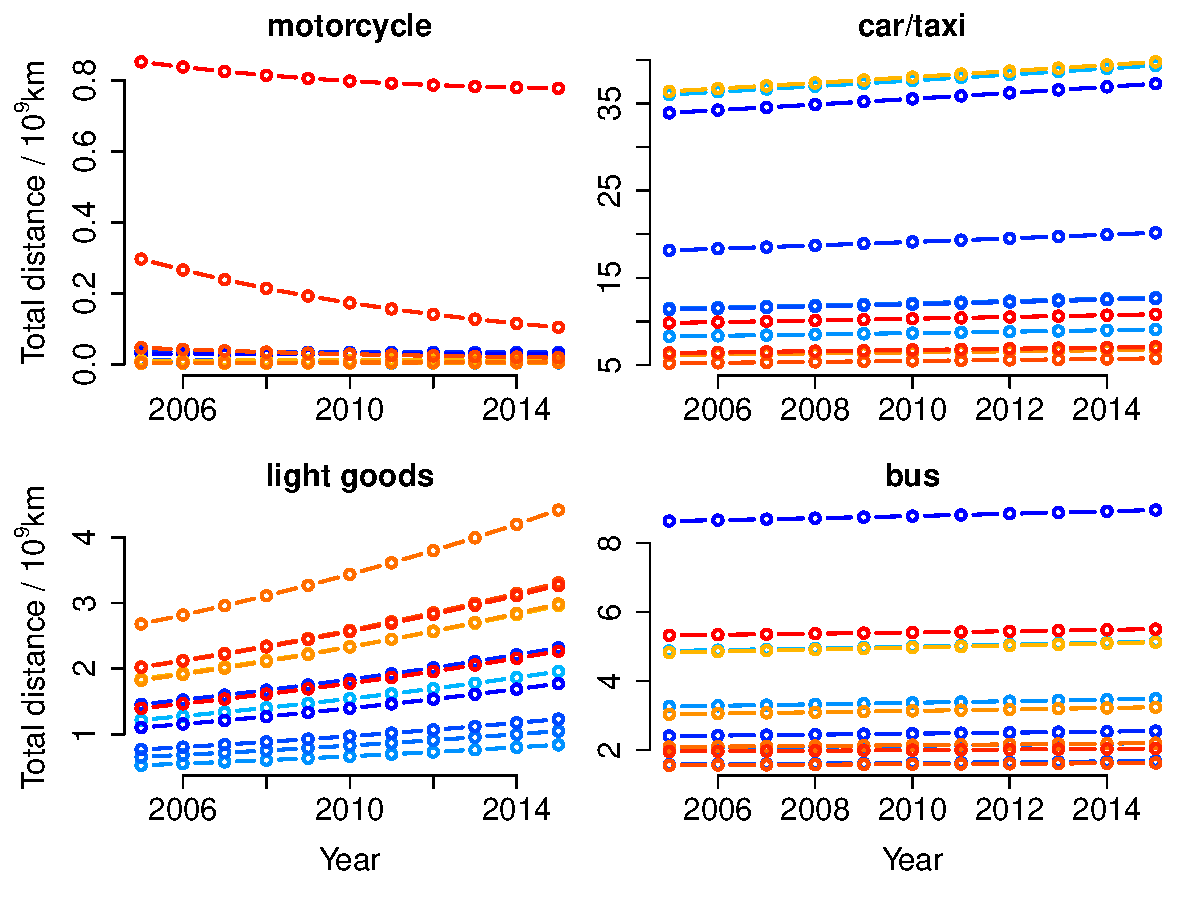
\includegraphics[width=0.45\textwidth]{passSmooth.pdf}&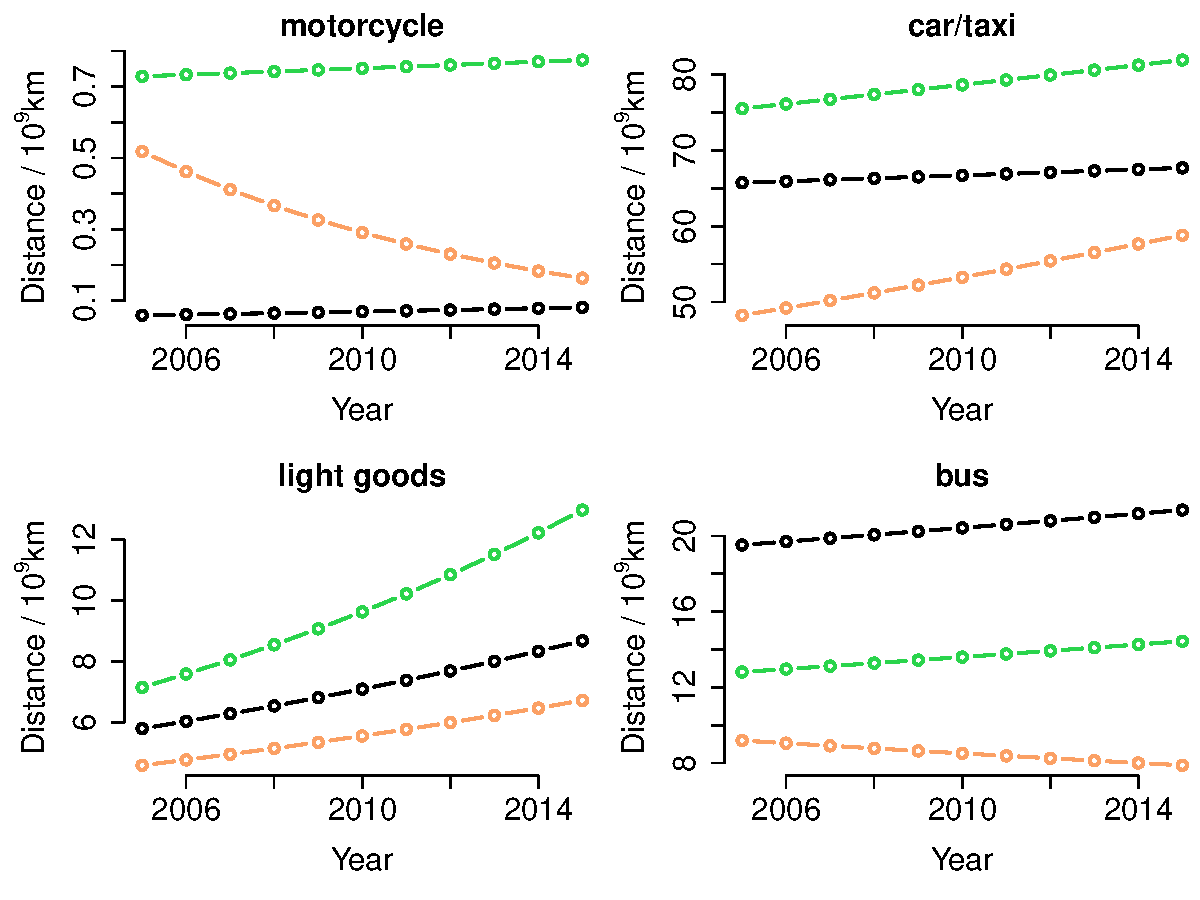
\includegraphics[width=0.45\textwidth]{roadPassSmooth.pdf}
\end{tabular}
\caption{\small Smoothed data: passengers.}
\label{smoothpass}
\end{figure}

%\section{Safety in numbers}

%Safety in numbers is the principle that the expected number of injuries is not necessarily linearly related to the volume of road traffic. It might be that an increase in road traffic by a certain proportion is not followed by an increase in road-traffic injuries by the same proportion.

%Mathematically, we describe the relationship as follows \citep{Elvik2017}:
%\begin{equation}\label{original}
%\text{Number of injuries} = e^{\beta_0}N_{(\text{str})}^{\beta_1}N_{(\text{cas})}^{\beta_2}\exp\left(\sum_{i=3}^n\beta_iX_i\right)
%\end{equation}
%where $N_{(\text{str})}$ is the annual average daily traffic (AADT) volume of the striking vehicle and $N_{(\text{cas})}$ is the AADT volume of the casualty vehicle. $\beta_i$ are coefficients fit to data, and $X_i$ is the (any) model matrix. The safety-in-numbers exponents are $\beta_1$ and $\beta_2$. For $\beta_1=1$ or $\beta_2=1$, we see that injuries are linear in terms of striker or victim volume, respectively. If $\beta_1<1$ or $\beta_2<1$, we see that there is ``safety in numbers'', in that additional road users do not increase the number of injuries in line with (linearly with) the extent of road-user inflation.

%We rewrite this equation, specific to the two modes and making explicit the specificity to road type and year, as\footnote{Omitted indices are marginalised. $m'$ denotes that the striker vehicle might be different from the casualty vehicle, $m$.}
%\begin{equation}\label{original}
%\log\left(\text{Number of injuries}\right) = {\beta_0} + {\beta_1}\log\left(N_{m',t,y}^{(\text{str})}\right)+{\beta_2}\log\left(N_{m,t,y}^{(\text{cas})}\right)+\sum_{i=3}^n\beta_iX_i
%\end{equation}

%\subsection{Safety in numbers: example}

%We can write this as the rate of injuries per striker vehicle per casualty vehicle:
%\begin{equation}\label{number}
%\log\left(\begin{tabular}{c}\text{Number of injuries per striking}\\\text{vehicle per casualty vehicle}\end{tabular}\right)= {\beta_0} + ({\beta_1}-1)\log\left(N_{m',t,y}^{(\text{str})}\right)+({\beta_2}-1)\log\left(N_{m,t,y}^{(\text{cas})}\right)+\sum_{i=3}^n\beta_iX_i.
%\end{equation}

%Then we can express the injury number for specific subgroups based on their travel patterns, e.g. for female travellers with AADT volume $N_{F,m,t,y}^{(\text{cas})}$:
%\begin{equation}
%\log\left(\begin{tabular}{c}\text{Number of injuries}\\\text{of female travellers}\\\text{per motorised vehicle}\end{tabular}\right) = \log(N_{F,m,t,y}^{(\text{cas})})+{\beta_0} + ({\beta_1}-1)\log\left(N_{m',t,y}^{(\text{str})}\right)+({\beta_2}-1)\log\left(N_{m,t,y}^{(\text{cas})}\right)+\sum_{i=3}^n\beta_iX_i.
%\end{equation}




%\subsection{Safety in distance}

%Our exposure data for road users are in the form of total distances travelled in kilometres in a year. We denote these values $A_{m,t,y}^{\text{(str)}}$ and $A_{m,t,y}^{\text{(cas)}}$ for total annual distance travelled by striker and casualty vehicle, respectively. 

%So we want to transform Equation \ref{original} into the rate of injuries per striker vehicle distance per casualty vehicle distance (instead of injuries per number, as in Equation \ref{number}):

%\begin{align}
%\log\left(\begin{tabular}{c}\text{Number of injuries per}\\\text{striker vehicle distance per}\\\text{casualty vehicle distance}\end{tabular}\right) = {\beta_0} +& {\beta_1}\log\left(N_{m',t,y}^{(\text{str})}\right)-\log(A_{m',t,y}^{\text{(str)}})+\nonumber\\
%&{\beta_2}\log\left(N_{m,t,y}^{(\text{cas})}\right)-\log(A_{m,t,y}^{\text{(cas)}})+\sum_{i=3}^n\beta_iX_i
%\end{align}



%Then we can estimate the number of injuries for female travellers given the total distance they cover, $A_{F,m,t,y}^{\text{(cas)}}$:
%\begin{align}
%\log\left(\begin{tabular}{c}\text{Number of injuries of}\\\text{female travellers per}\\\text{striker vehicle distance}\end{tabular}\right) = \log(A_{F,m,t,y}^{\text{(cas)}})+&{\beta_0} +{\beta_1}\log\left(N_{m',t,y}^{(\text{str})}\right)-\log(A_{m',t,y}^{\text{(str)}})+\nonumber\\
%&{\beta_2}\log\left(N_{m,t,y}^{(\text{cas})}\right)-\log(A_{m,t,y}^{\text{(cas)}})+\sum_{i=3}^n\beta_iX_i
%\end{align}

%We  can estimate $N_{m,t,y}^{(\text{str})}$ and $N_{m,t,y}^{(\text{cas})}$ as the average daily number of trips according to the NTS data. Each trip in the NTS dataset has a weight, $w_j$. This weight encompasses the weight of the person, and we upweight the weight by $\rho_{m,y}$. Then the total numbers of journeys are
%\begin{align}
%N_{m,t,y}^{(\text{cas})} &= \rho_{m(j),y(j)} \smashoperator{\sum_{\substack{j:m(j)=m,\\y(j)=y,D_{j,t}>0}}}w_{j}/365,\\
%N_{m,t,y}^{(\text{str})} &= \rho_{m(j),y(j)} \smashoperator{\sum_{\substack{j:m(j)=m,\\y(j)=y,z(j)=0\\D_{j,t}>0}}}w_{j}/365.
%\end{align}

%To calculate the number of bus journeys, we assume that the ratio of bus trips to bus passenger trips is the same as the ratio of bus distance to bus passenger distance:
%\begin{equation}
%N_{m=\text{bus},t,y,z=0} = N_{m=\text{bus},t,y,z=1}\frac{A_{m=\text{bus},t,y,z=0}}{A_{m=\text{bus},t,y,z=1}}.
%\end{equation}

%For HGVs, we estimate the mean journey distance to be 98 km,\footnote{\url{http://ec.europa.eu/eurostat/statistics-explained/index.php/Road_freight_transport_by_journey_characteristics}} and therefore the average trip number as:
%\begin{align}
%N_{m=\text{HGV},t,y}^{(\text{cas})} &= N_{m=\text{HGV},t,y}^{(\text{str})} \\
% &= A_{m=\text{HGV},t,y}^{(\text{str})}/98/365.
%\end{align}

%\subsection{Concern}

%Let's return to Equation \ref{original}. The exponents, $\beta_1$ and $\beta_2$, are found by fitting observed counts of individuals and collisions at specific points in roads or junctions.

%In our case, we are considering many roads and junctions simultaneously -- all the roads and junctions in England. Let's imagine that we are just considering two sites. We would expect:
%\begin{equation}
%\text{Number of injuries at site 1} = e^{\beta_0}N_{(\text{str,1})}^{\beta_1}N_{(\text{cas,1})}^{\beta_2}\exp\left(\sum_{i=3}^n\beta_iX_i\right)
%\end{equation}
%\begin{equation}
%\text{Number of injuries at site 2} = e^{\beta_0}N_{(\text{str,2})}^{\beta_1}N_{(\text{cas,2})}^{\beta_2}\exp\left(\sum_{i=3}^n\beta_iX_i\right)
%\end{equation}
%In total, we should have
%\begin{equation}\label{independent}
%\text{Number of injuries} = e^{\beta_0}\left(N_{(\text{str,1})}^{\beta_1}N_{(\text{cas,1})}^{\beta_2}+N_{(\text{str,2})}^{\beta_1}N_{(\text{cas,2})}^{\beta_2}\right)\exp\left(\sum_{i=3}^n\beta_iX_i\right)
%\end{equation}
%but, according to our model, what we are actually calculating is
%\begin{equation}\label{summed}
%\text{Number of injuries} = e^{\beta_0}\left(N_{(\text{str,1})}+N_{(\text{str,2})}\right)^{\beta_1}\left(N_{(\text{cas,1})}+N_{(\text{cas,2})}\right)^{\beta_2}\exp\left(\sum_{i=3}^n\beta_iX_i\right).
%\end{equation}
%However, $N_{(\text{str,1})}^{\beta_1}N_{(\text{cas,1})}^{\beta_2}+N_{(\text{str,2})}^{\beta_1}N_{(\text{cas,2})}^{\beta_2}\neq\left(N_{(\text{str,1})}+N_{(\text{str,2})}\right)^{\beta_1}\left(N_{(\text{cas,1})}+N_{(\text{cas,2})}\right)^{\beta_2}$.

%\begin{figure}[H]
%\centering
%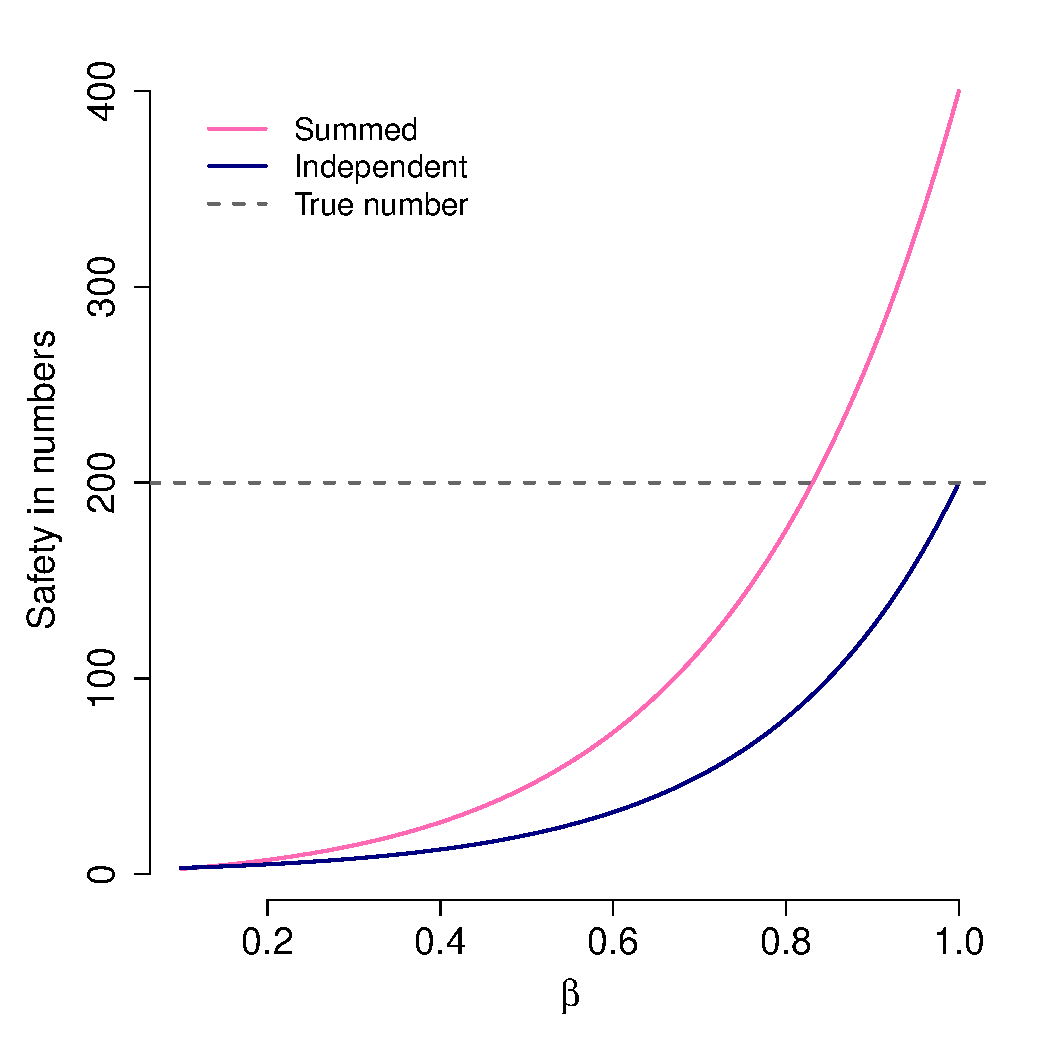
\includegraphics[width=0.6\textwidth]{sinsum.pdf}
%\caption{\small Realisations of Equations \ref{independent} (independent) and \ref{summed} (summed), for $\beta=\beta_1=\beta_2$ and $N_{(\text{cas,1})}=N_{(\text{cas,2})}=N_{(\text{str,1})}=N_{(\text{str,2})}=10$. The true number of interacting road users is shown in dashed gray ($2N^2$). The summed estimate (pink) overestimates the observed safety-in-numbers effect (navy).}
%\label{descriptive}
%\end{figure}


\section{Casualties}\label{injuries}

The Stats19 database lists 2,137,625 road-traffic injuries and fatalities for the years 2005--2015. We process these data in order to group the casualties according to nine predictors: year, striker age, casualty age, road type, strike mode, casualty mode, casualty gender, casualty severity, striker gender. Note that the Stats19 database does not distinguish between casualties and strikers: we define these ourselves in processing the data, choosing the largest party as the striking mode. Their marginal distributions are shown in Figure \ref{descriptive}.

\begin{figure}[H]
\centering
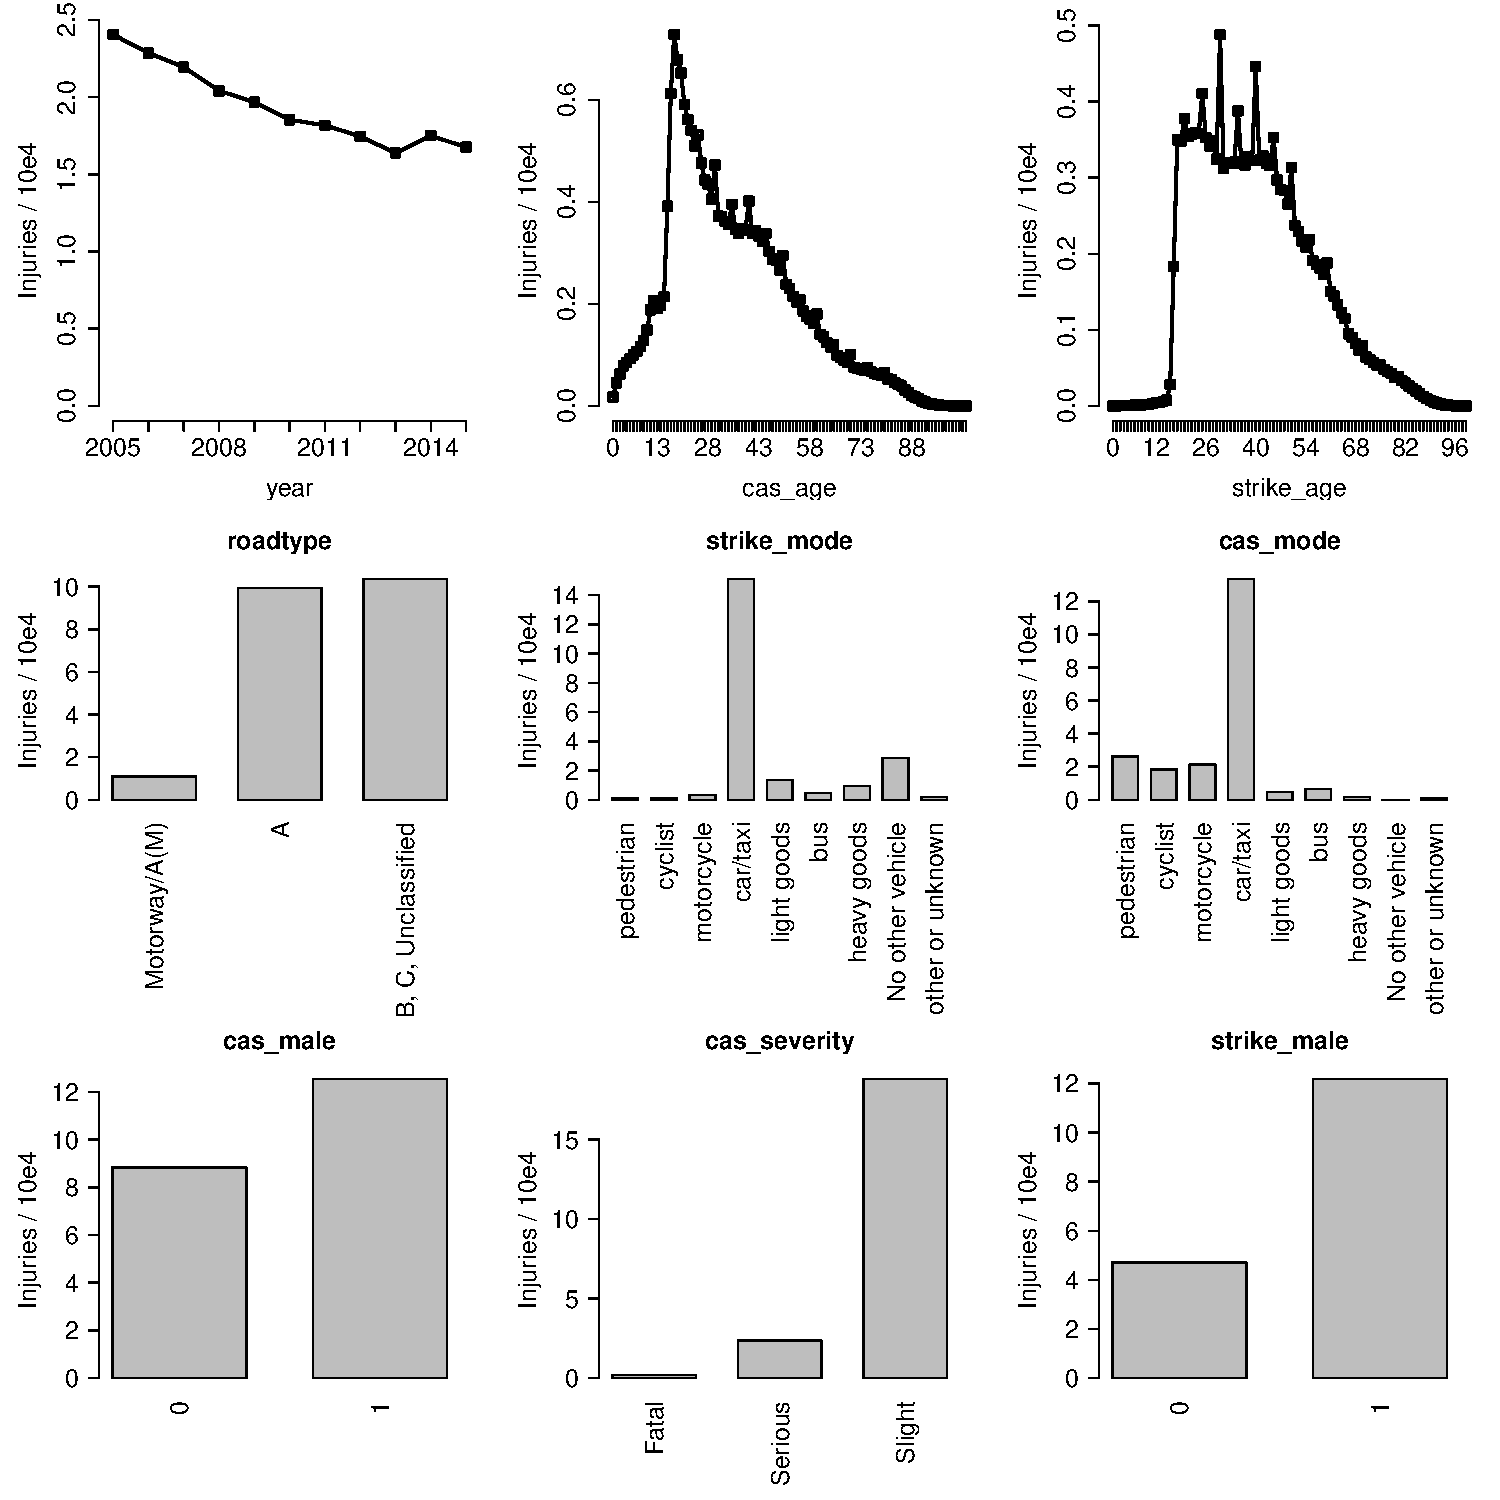
\includegraphics[width=0.6\textwidth]{descriptive.pdf}
\caption{\small Marginal distributions of all casualties in the Stats19 database from 2005 to 2015.}
\label{descriptive}
\end{figure}

Before proceeding, we omit any entries with missing data, which includes any entry with modes ``no other vehicle'' or ``other or unknown''. Then 1,473,533 entries remain. We have a separate model for ``no other vehicle'' that includes data from other sources.

Finally, we select age groupings for both the casualty and striker ages, so that the number of age groups is reduced from 106 to 6 for each. The reduced number of groups allows for greater computational efficiency. Age groups are chosen as the quantiles extracted from the data shown in Figure \ref{descriptive}.

%\section{Missing data}

\section{Regression modelling}\label{regression}

We seek to build a model for estimating the number of casualties sustained by road users by fitting a negative binomial model to data from the Stats19 database. We make estimates for each combination of: casualty severity, road type, year, strike mode, casualty mode, striker demographic group, and casualty demographic group. The number of casualties in each group is assumed to follow a negative binomial distribution with its own rate, $\lambda$. The covariates determine the rate $\lambda$ in fitting the model. Thus we say that $\lambda$ is parametrised by the covariates.

We use regression to estimate the number of casualties per distance travelled in order to smooth the casualty data. Our disaggregation of the data results in many counts of zero. Smoothing allows the sharing of support across similar groups. Note that distance data were smoothed prior to regression.

\subsection{Negative binomial equation}

\hl{[EITHER]}

We augment the Stats19 dataset by adding to each year-mode-road-demographic group their distance travelled ($A_{a,g,m,t,y}^{\text{(cas)}}$ and $A_{a',g',m',t,y}^{\text{(str)}}$), the safety-in-numbers exponents ($\beta_1$ and $\beta_2$), the AADF ($N_{m,t,y}^{\text{(cas)}}$ and $N_{m',t,y}^{\text{(str)}}$) and the distance travelled by AADF groups ($A_{m,t,y}^{\text{(cas)}}$ and $A_{m',t,y}^{\text{(str)}}$). Here, the age groups, $a$ and $a'$, are those defined in Section \ref{injuries}.

Then we have all components for the model defined as
\begin{align}
I_{a,a',m,m',g,g',c,t,y}&\sim \text{NB}(\lambda_{a,a',m,m',g,g',c,t,y},\theta) \\
\log\left(\lambda_{a,a',m,m',g,g',c,t,y}\right) &= {\beta_0} +\log(A_{a,g,m,t,y}^{\text{(cas)}})+{\beta_1}\log\left(N_{m',t,y}^{(\text{cas})}\right)-\log(A_{m',t,y}^{\text{(cas)}})+\nonumber\\
&\quad\log(A_{a',g',m',t,y}^{\text{(str)}})+{\beta_2}\log\left(N_{m',t,y}^{(\text{str})}\right)-\log(A_{m',t,y}^{\text{(str)}})+\sum_{i=3}^n\beta_iX_i.
\end{align}

The parameters $\beta_1$ and $\beta_2$ are safety-in-numbers exponents. They represent the non-linearity in the relation between distance travelled and number of casualties incurred \citep{Aldred2017,Elvik2017}. 

\hl{[OR]}

We augment the Stats19 dataset by adding to each year-mode-road-demographic group their distance travelled ($A_{a,g,m,t,y}^{\text{(cas)}}$ and $A_{a',g',m',t,y}^{\text{(str)}}$). Here, the age groups, $a$ and $a'$, are those defined in Section \ref{injuries}.

Then we have all components for the model defined as
\begin{align}
I_{a,a',m,m',g,g',c,t,y}&\sim \text{NB}(\lambda_{a,a',m,m',g,g',c,t,y},\theta) \\
\log\left(\lambda_{a,a',m,m',g,g',c,t,y}\right) &= {\beta_0} +\log(A_{a,g,m,t,y}^{\text{(cas)}})+\log(A_{a',g',m',t,y}^{\text{(str)}})+\sum_{i=1}^n\beta_iX_i.
\end{align}

We omit safety-in-numbers exponents on the basis that there are no published coefficients appropriate to a country-level dataset, and our dataset is insufficient to learn them directly \citep{Aldred2017,Elvik2017}. We show in supplementary material the model that results when we try to learn these as additional parameters (?).



\hl{[END]}

The model matrix is represented by $X$ and $\beta$ are the coefficients to fit. In fitting, we remove from the dataset any entries for which $A_{a,g,m,t,y}^{\text{(cas)}}$ or $A_{a',g',m',t,y}^{\text{(str)}}$ is zero. This takes us from 698,544 unique combinations to 580,536. 


\subsection{Model building}

All covariates we might use are listed at the beginning of Section \ref{injuries}. In addition to using these as predictors alone, we use interactions between them as covariates. To begin, we choose which pairs, triplets, and quadruplets of interacting covariates to include in parametrising the rate parameter $\lambda$.

To build the negative binomial regression model, we start from the main-effects model (which consists of nine covariates as predictors, and no interactions), and add one interaction at a time. The ``year'' covariate is modelled as a smooth spline with two knots, and both age variables are modelled as a smooth spline with knots at each age median. 

We aim to minimise Akaike's information criterion (AIC) \citep{Akaike1983} in the model we build. This metric quantifies goodness of fit with an accompany penalty for the complexity of the model, proxied by the number of parameters.

The algorithm is:
\begin{enumerate}
\item Set $\mathcal{M}$ as the nine main-effects model
\item Define the set of possible additional interactions $\mathscr{I}$
\item Calculate AIC for all models $\mathcal{M+I}$ where $\mathcal{I}\in\mathscr{I}$
\item \textbf{while} $\min_{\mathscr{I}}\text{AIC}(\mathcal{M+I})<\text{AIC}(\mathcal{M})$ \textbf{do:}
\begin{enumerate}
\item Set $\mathcal{M}\leftarrow\mathcal{M+I^*}$, where $\mathcal{M+I^*}$ is the model with minimal AIC
\item Redefine the set of possible additional interactions $\mathscr{I}$
\item Calculate AIC for all models $\mathcal{M+I}$ where $\mathcal{I}\in\mathscr{I}$
\end{enumerate}
\item\textbf{end while}
\end{enumerate}

The ``set of possible additional interactions $\mathscr{I}$'' are those those up to order $n=3$, subject to the condition that all interactions of order $n-1$ that are contained in $\mathcal{I}$ already exist in $\mathcal{M}$. Thus, it is a forward selection algorithm to build an interaction hierarchy model.

We cease building the model at the point at which the AIC begins increasing. For the NOV model, this is after 27 additions.

\section{Results: estimated rates / fit to data}\label{results}

We plot some results for certain sections of the set in Figures \ref{NOVpredYear}--\ref{pred6Age2015MC}. Predictions are summed over each subgroup and plotted for each gender and each road type. Raw estimates are faded in the background.

These plots highlight some problems with the distance data. E.g., there is a very high rate of females injured on motorcycles on motorways in crashes with no other vehicle (Figure \ref{NOVpredAge2015}). This can be explained by the estimation that a very small distance is travelled on motorways, combined with a small expected number of casualties. The result is that the rate is very high. The same problem is apparent in the heavy goods panel of the same figure.

\begin{figure}[H]
\centering
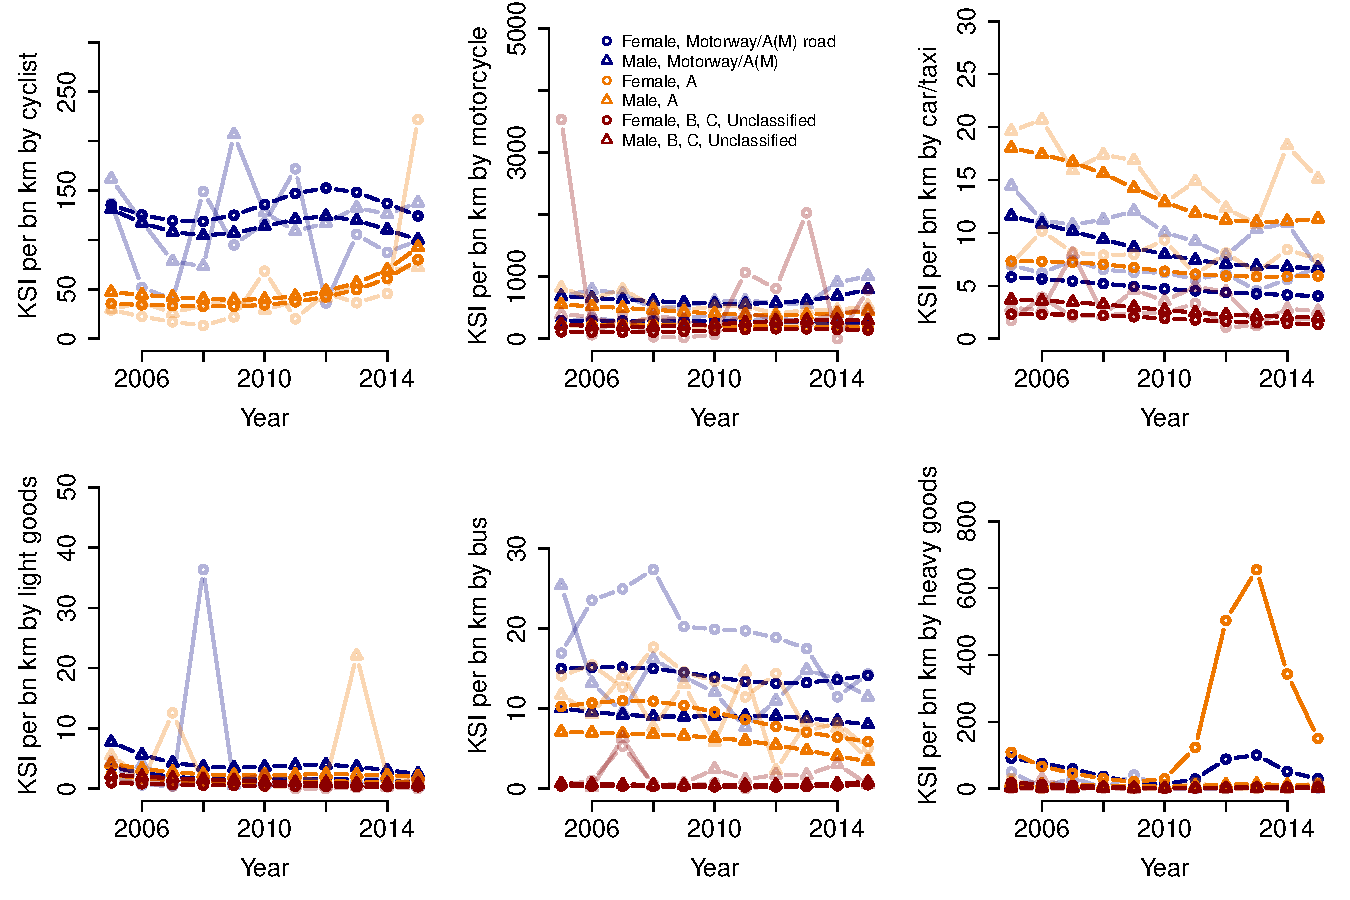
\includegraphics[width=0.6\textwidth]{NOVpredYearKSI.pdf}
\caption{\small Mean casualty rate caused by no other vehicle for each year.}
\label{NOVpredYear}
\end{figure}

\begin{figure}[H]
\centering
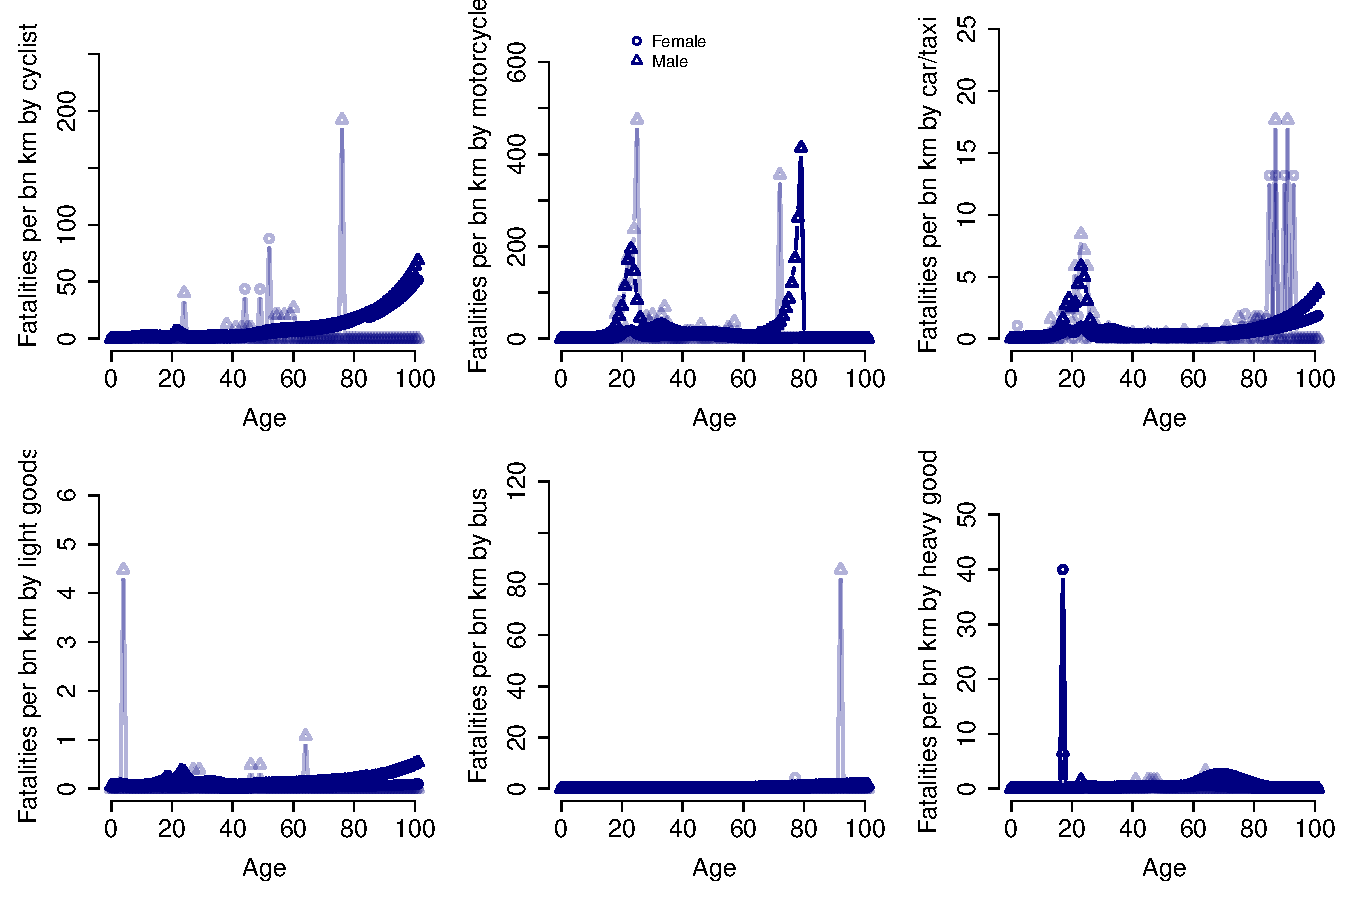
\includegraphics[width=0.6\textwidth]{NOVpredAge2015sumFatalities.pdf}
\caption{\small Sum of fatalities caused by no other vehicle for each casualty age group in 2015.}
\label{NOVpredAge2015}
\end{figure}

\begin{figure}[H]
\centering
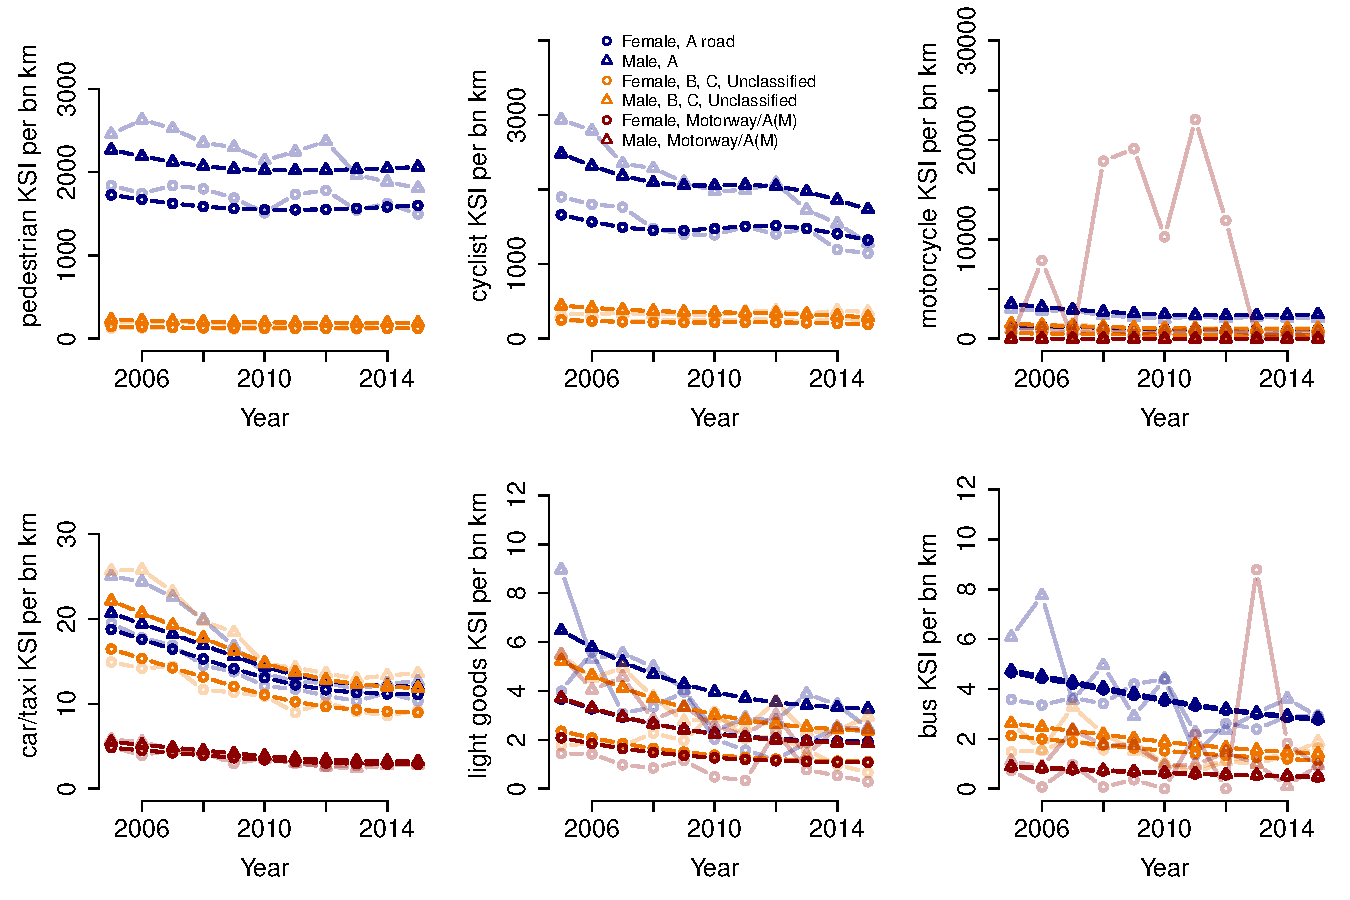
\includegraphics[width=0.6\textwidth]{pred6year.pdf}
\caption{\small Mean casualty rate caused by any vehicle for each year.}
\label{pred6year}
\end{figure}

\begin{figure}[H]
\centering
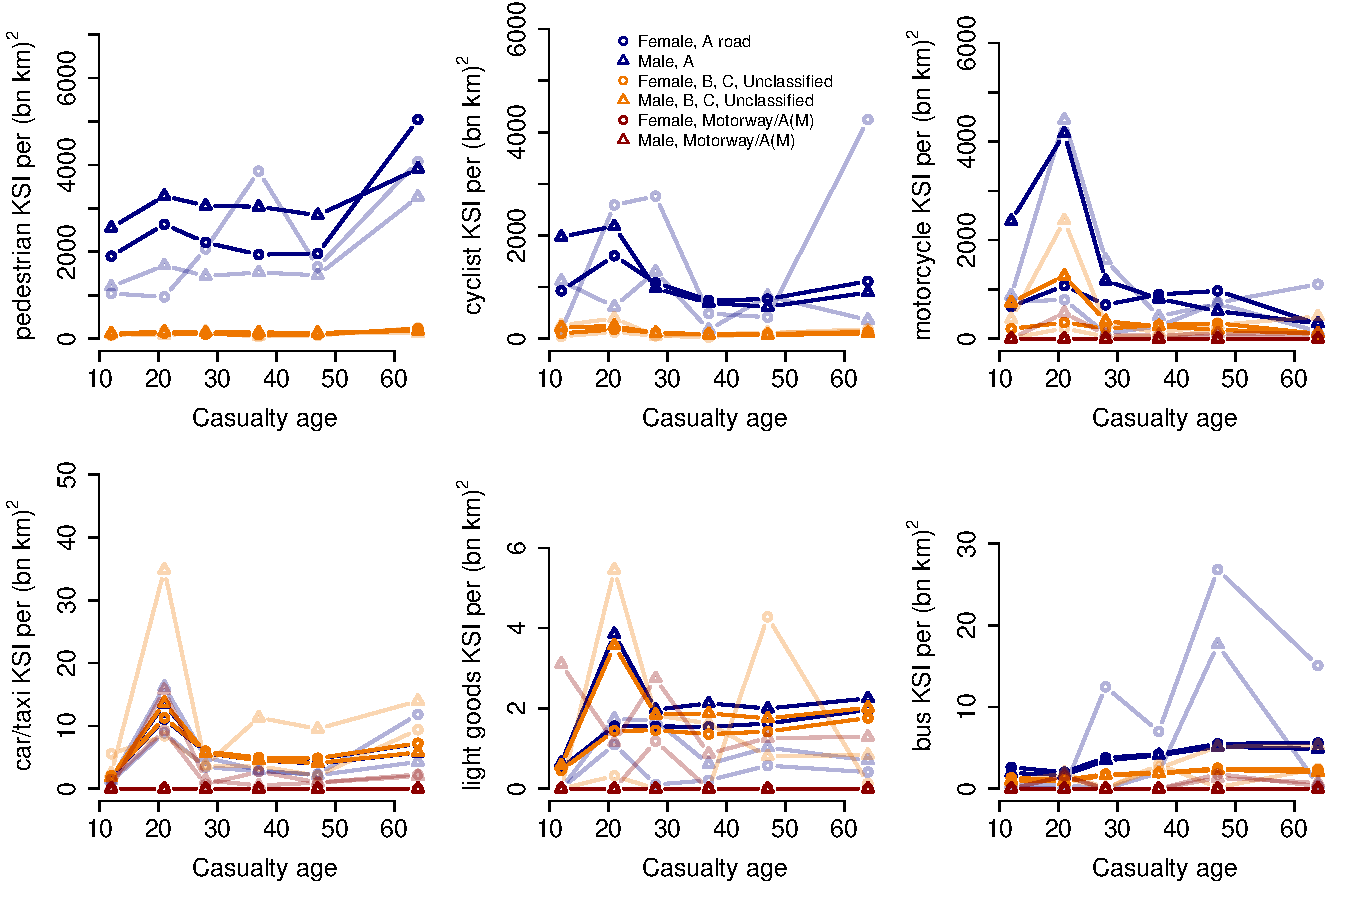
\includegraphics[width=0.6\textwidth]{pred6Age2015.pdf}
\caption{\small Sum of casualties caused by any vehicle for each casualty age group in 2015.}
\label{pred6Age2015}
\end{figure}

\begin{figure}[H]
\centering
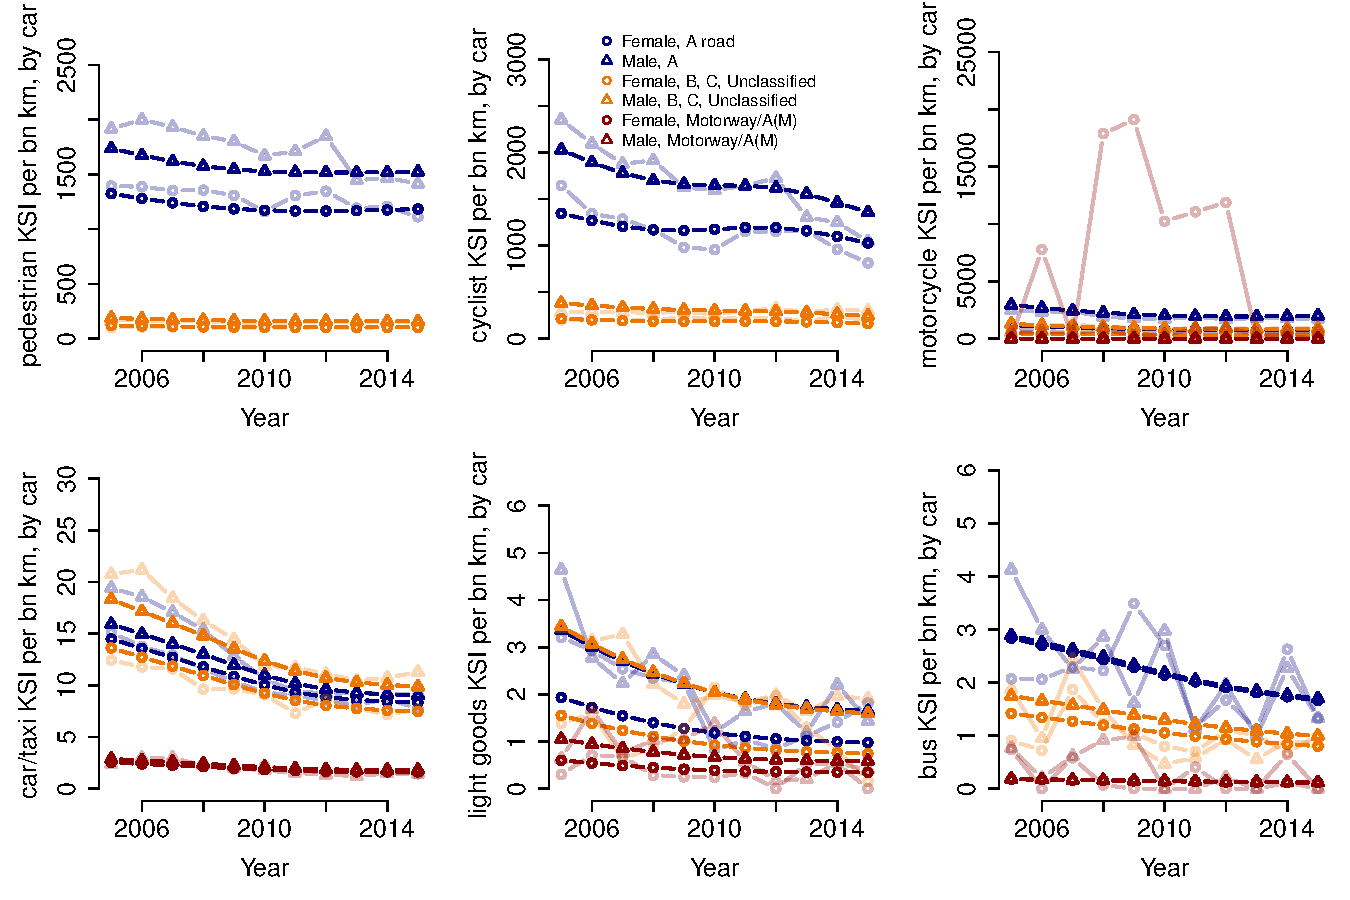
\includegraphics[width=0.6\textwidth]{pred6yearCar.pdf}
\caption{\small Mean casualty rate caused by car for each year.}
\label{pred6yearCar}
\end{figure}

\begin{figure}[H]
\centering
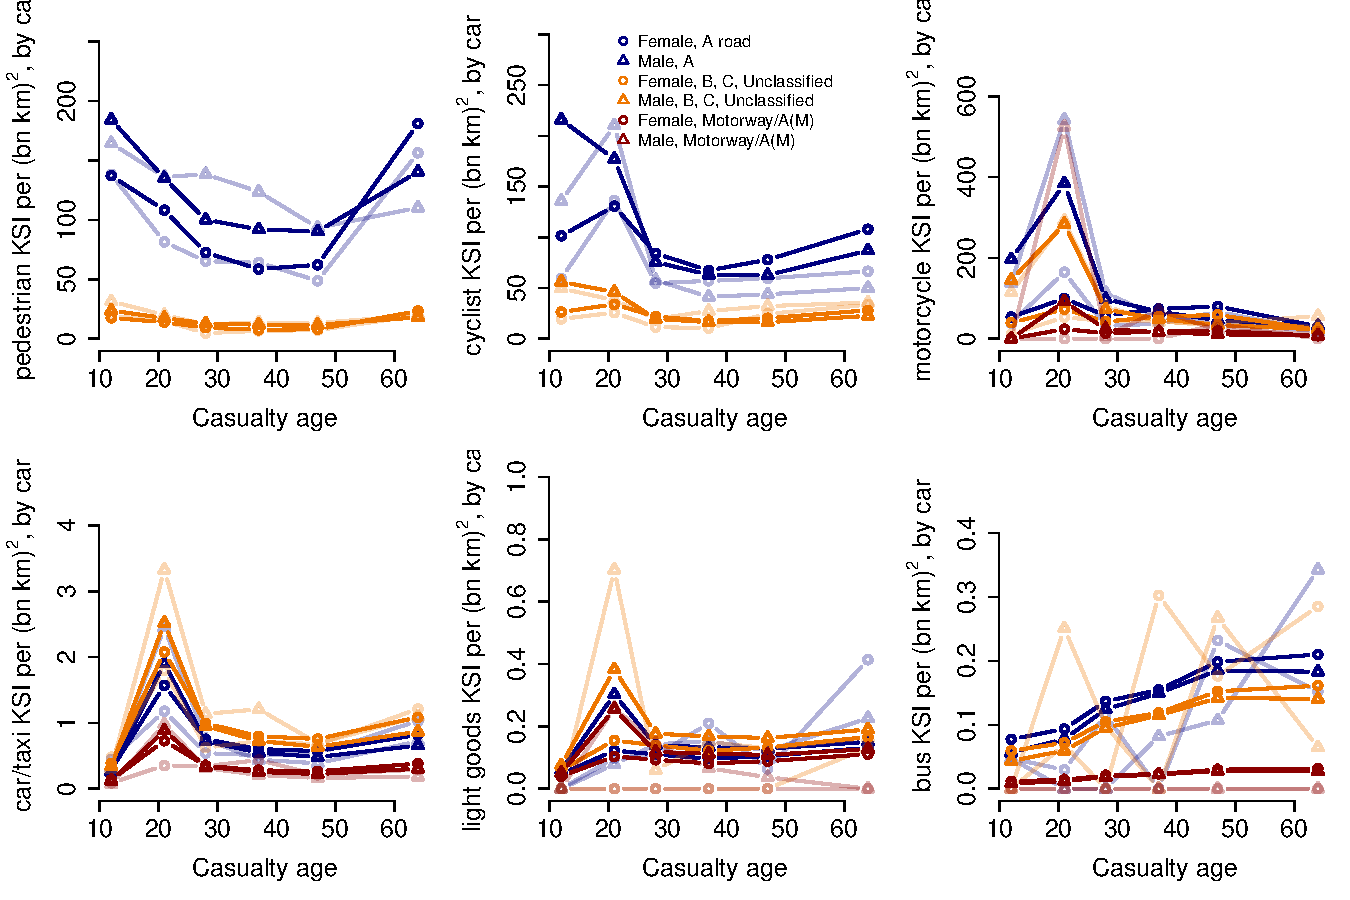
\includegraphics[width=0.6\textwidth]{pred6Age2015Car.pdf}
\caption{\small Sum of casualties caused by car for each casualty age group in 2015.}
\label{pred6Age2015Car}
\end{figure}

\begin{figure}[H]
\centering
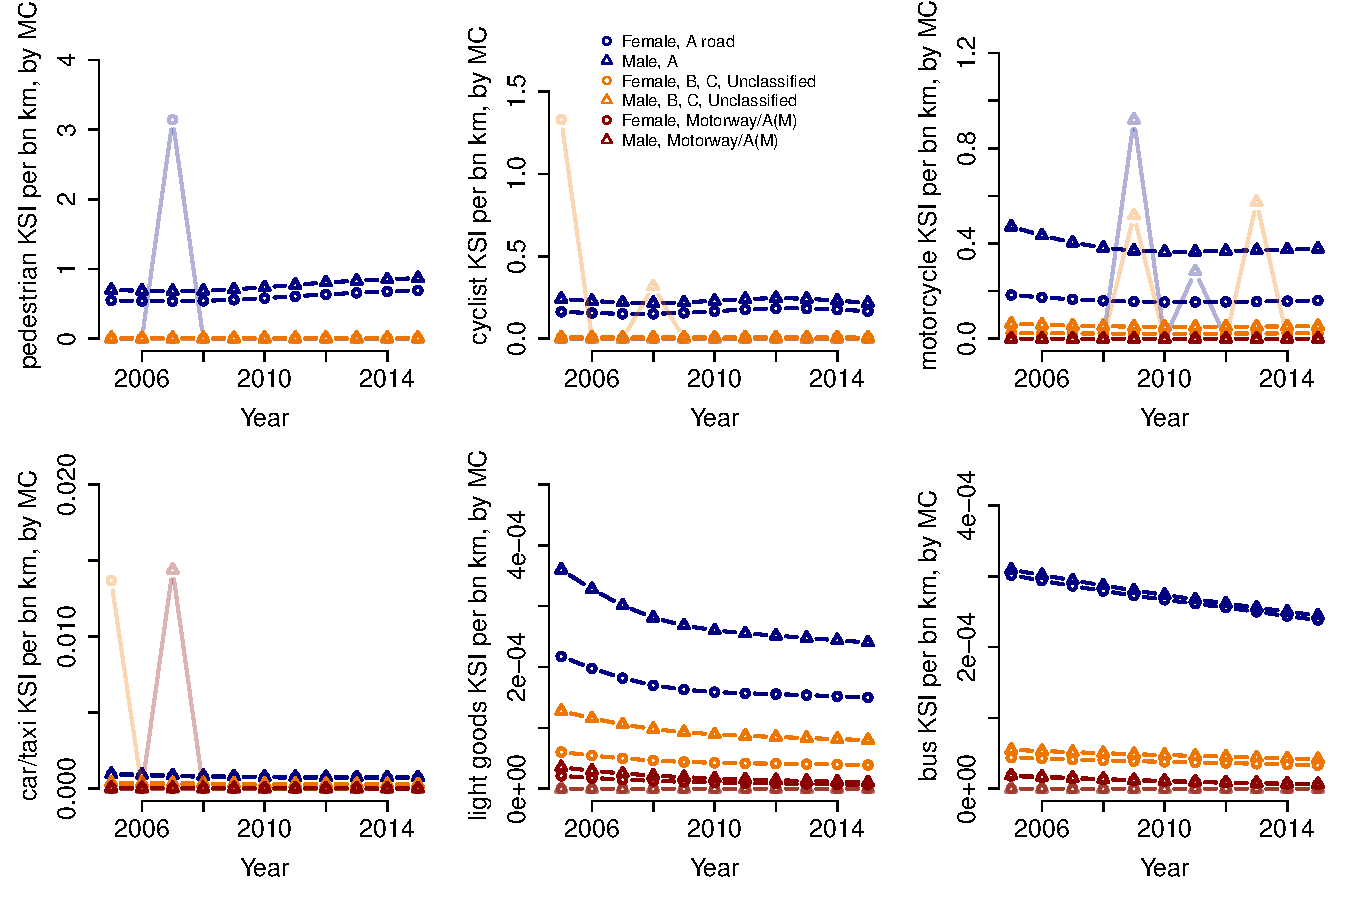
\includegraphics[width=0.6\textwidth]{pred6yearMC.pdf}
\caption{\small Mean strike rate by female motorcyclists for each year.}
\label{pred6yearMC}
\end{figure}

\begin{figure}[H]
\centering
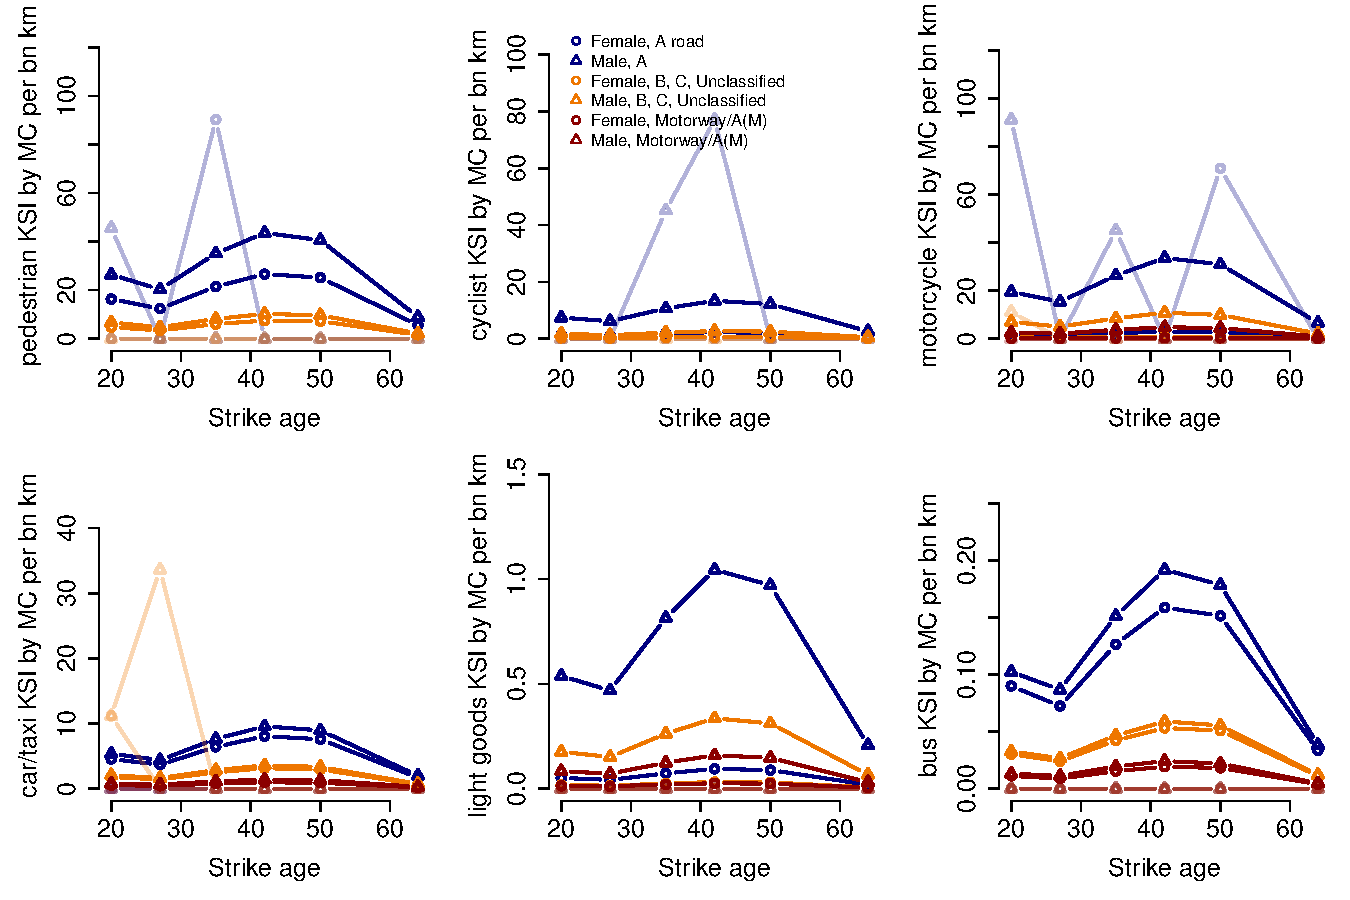
\includegraphics[width=0.6\textwidth]{pred6Age2015MC.pdf}
\caption{\small Sum of casualties caused by female motorcyclists for each striker age group in 2015.}
\label{pred6Age2015MC}
\end{figure}

\section{Predictions for novel scenarios}

We make predictions for the baseline by constructing what we believe to be the baseline travel distances, i.e. the true amount of travel currently undertaken, and predicting the number of casualties using the predictive model. These distances might be the same as the offset in the fitted model, or calculated in the same way. %It could be a sum over the synthetic population.

To make predictions for supposed scenarios, we create a new distance-travelled array, ${C}_{a,g,m,t,y,z,s}$, to reflect the scenario-specific travel behaviour. The new index $s$ denotes the scenario. $C$ is equivalent to $\tilde{B}$; indeed, we might have ${C}_{a,g,m,t,y,z,s_0}=\tilde{B}_{a,g,m,t,y,z}$, where $s=s_0$ denotes the baseline.

We can create $C$ for a new scenario by re-allocating the distance travelled, $D_j$, for every journey that changes mode from baseline to scenario. For baseline journey  $j_{s_0}$  and scenario journey $j_s$, with modes $m(j_{s_0})$ and $m(j_s)$ and distances on each road are $f_{m(j_{s_0}),t}(D_{j})$ and $f_{m(j_s),t}(D_{j})$, we add the distance to the new scenario and subtract from the baseline as follows:
$${C}_{a(j),g(j),m(j_s),t,y(j),z(j),s} = {C}_{a(j),g(j),m(j_s),t,y(j),z(j),s_0}+f_{m(j_s),t}(D_{j}),$$
$$C_{a(j),g(j),m(j_{s_0}),t,y(j),z(j),s} = C_{a(j),g(j),m(j_{s_0}),t,y(j),z(j),s_0}-f_{m(j_{s_0}),t}(D_{j}).$$

The general formula for application of this to all items in the distance array is:
$${C}_{a,g,m,t,y,z,s} = {C}_{a,g,m,t,y,z,s_0}\;+\;\smashoperator{\sum_{\substack{j:a(j)=a,\\g(j)=g,m(j_s)=m,\\m(j_{s_0})\neq m,\\y(j)=y,z(j)=z}}}\;f_{m(j_s),t}(D_{j})\;-\;\smashoperator{\sum_{\substack{j:a(j)=a,\\g(j)=g,m(j_s)\neq m,\\m(j_{s_0})= m,\\y(j)=y,z(j)=z}}}\;f_{m(j_{s_0}),t}(D_{j}).$$




\clearpage
% \begin{minipage}[l]{0.5\linewidth}
% \tikz{ %
%     \node[latent] (x) {$x_{d(j),m,z}$} ; %
%     %\node[latent, right=of x,xshift=2cm] (mu) {$\mu_{d,m,z}$} ; %
%     \node[obs, above=of x] (n) {$n_{j,m,z}$} ; %
%     \node[latent, above=of n] (lambda) {$\lambda_{d(j),m,z}$} ; %
%     %\node[latent, left=of n] (xhat) {$\hat{x}_{j,m,z}$} ; %
%     \node[latent, right=of n,xshift=1cm] (muhat) {$\hat{\mu}_{j,m,z}$} ; %
%     \node[obs, above=of muhat] (D) {$D_{j,m,z}$} ; %
%     \node[latent, below=of muhat] (r) {$r_{d(j),m,z,t}$} ; %
%     \node[obs, right=of r,xshift=0.5cm] (R) {$R_{m,y,t}$} ; %
%     \node[latent, below=of r] (B) {$B_{d(j),m,z,t}$} ; %
%     \plate[inner sep=0.25cm, xshift=-0.12cm, yshift=0.12cm]{plate2} {(B) (R)} {$t\in\{M,A,B\}$};
%     {\tikzset{plate caption/.append style={below right=0pt and 0pt of #1.south west}}\plate[inner sep=0.25cm, xshift=0.12cm, yshift=0.12cm]{plate1} {(D) (x) (lambda) (B)} {$z,j$}}; 
%     {\tikzset{plate caption/.append style={below right=0pt and 0pt of #1.south west}}\plate[inner sep=0.25cm, xshift=0.12cm, yshift=0.12cm]{plate3} {(plate2) (plate1)} {$m$}}; 
%     \edge {lambda} {n} ;
%     %\edge {xhat} {x} ;
%     \edge {muhat} {D,r,x} ;
%     \edge {n} {muhat,x,D,r} ;
%     %\edge {mu} {r} ;
%     \edge {r} {R} ;
%     \edge {r,x} {B} ;
%   }
% \end{minipage}
% \begin{minipage}[l]{0.4\linewidth}
% \begin{align*}
% d=&\{a,g,y\}\\
% j=&\text{individual}\\
% a=&\text{age}\\
% g=&\text{gender}\\
% y=&\text{year}\\
% m=&\text{mode}\\
% z=&\text{passenger}\\
% D=&\text{Set of trips}\\
% x=&\text{total travel per person}\\
% n=&\text{number of trips per person}\\
% \mu=&\text{trip distance}\\
% r=&\text{trip distributed to road type}\\
% R=&\text{RTS data}\\
% B=&\text{Target smoothed distances}\\
% \end{align*}
% \end{minipage}
% \bigskip


% We are interested in the dataset $D_{j,m,z}$: the set of trips made by individual $j$ by mode $m$ as a passenger or not ($z$).

% Each individual makes $n_{j,m,z}$ trips for mode combination $\{m,z\}$:
% $$ n_{j,m,z}|\lambda_{d(j),m,z}\sim \text{NB}(\lambda_{d(j),m,z},\cdot).$$
% In terms of the NTS dataset,
% $$ \text{dim}(D_{j,m,z})|\lambda_{d(j),m,z}\sim \text{NB}(\lambda_{d(j),m,z},\cdot).$$

% The lengths of each person's trips depend on the number of trips made by that person:
% $$ \hat{\mu}_{j,m,z}|n_{j,m,z},\alpha_{d(j),m,z} \sim\mathcal{N}(\alpha_{1,d(j),m,z}(\alpha_{2,d(j),m,z}-n_{j,m,z}),\cdot).$$
% Together these define a distribution for trip length for each demographic group:
% $$\mu_{d(j),m,z} = \left\{\begin{array}{ll}
% 0&n_{j,m,z}=0\\
% \sum_{n_{j,m,z}} \hat{\mu}_{j,m,z}p(n_{j,m,z})&n_{j,m,z}>0.\end{array}\right.$$
% This gives us the distribution of the set of distances travelled for a person $j$ in demographic group $d(j)$: 
% \begin{align*}
% D_{j,m,z}|n_{j,m,z},\mu_{d(j),m,z} &\sim \mathcal{F}(n_{j,m,z},\mu_{d(j),m,z});\\
% \mathcal{F}(n_{j,m,z},\mu_{d(j),m,z})&=\left\{\begin{array}{ll}
% 0&n_{j,m,z}=0\\
% \left\{\exp(\mu_{d(j),m,z})\right\}_{n_{j,m,z}}&n_{j,m,z}>0.\end{array}\right.
% \end{align*}
% %$$p(D_{j,m,z}|n_{j,m,z}) = \prod_{1}^{n_{j,m,z}}p(\mu_{d(j),m,z}).$$

% The distance travelled per person, $x$, is something akin to a compound negative binomial distribution, except we want dependence between $\hat{\mu}_j$ and $n_j$.
% $$x_{d(j),m,z}|n_{j,m,z} = \left\{\begin{array}{ll}
% 0&n_{j,m,z}=0\\
% \sum_{k=1}^{n_{j,m,z}}\hat{\mu}_{j_k,m,z}p(n_{j,m,z}=k)&n_{j,m,z}>0.\end{array}\right.  $$

% Then the distance travelled in a demographic group $d$ (for dataset $D$ with individuals $j$ with person weight $w_j$) is then
% $$\log\left(\frac{\sum_{j:d(j)=d}\sum_{k=1}^{n_{j,m,z}}D_{j_k,m,z}}{\sum_{j:d(j)=d}w_j}\right)\sim \mathcal{N}\left(\sum_{k=1}^{n_{j,m,z}}p(k)x_{d(j),m,z},\cdot\right)$$

%The probability of a set of observed trips is 
%$$p(D_{j,m,z}|n_{j,m,z},\hat{\mu}_{j,m,z}) = p(n_{j,m,z}=0)+\sum_{n_{j,m,z}}\prod_{k=1}^{n_{j,m,z}}p(n_{j,m,z}=k)p(\hat{\mu}_{j,m,z}=D_{j_k,m,z}) $$

%\begin{align*} p(\lambda_{m,z},n_{m,z},\hat{\mu}_{m,z},D_{m,z}) =& p(\lambda_{m,z})\cdot
%p(n_{m,z}|\lambda_{m,z})\cdot p(\hat{\mu}_{m,z}|n_{m,z})\cdot p(D_{m,z}|\hat{\mu}_{m,z},n_{m,z})\\
%=& p(\lambda_{d,m,z})\cdot
%\prod_jp(n_{j,m,z}|\lambda_{d,m,z})\cdot p(\hat{\mu}_{j,m,z}|n_{j,m,z})\cdot p(D_{j,m,z}|\hat{\mu}_{j,m,z},n_{j,m,z})\\ \end{align*}



\clearpage
\bibliographystyle{agsm}
\bibliography{ithim}

\end{document}
